\label{app:efficiency_studies_muon}

The muon efficiencies measured in Monte Carlo simulation and data as well as the scale 
factor are shown in Table \ref{tab:eff_mu_offline_Full2011} for the full 2011 data and in Tables 
\ref{tab:eff_mu_offline_Run2011A} and \ref{tab:eff_mu_offline_Run2011B} for 
the Run2011A and Run2011B datasets respectively. Figures \ref{fig:mu_selectionEfficiency_massfits_lowPt}
and \ref{fig:mu_selectionEfficiency_massfits_highPt} show the dimuon mass fit 
results from which the efficiency for the full 2011 dataset was extracted for
low $p_{T}$ and high $p_{T}$ muons respectively.



 \begin{table}[!ht]
 \begin{center} 
 \begin{tabular}{|c|c|c|c|}
 \hline
 $p_{T}$ / $\eta$ bin    &  Monte Carlo Efficiency    &  Data Efficiency   &  MC to Data Scale Factor \\   \hline           
$ 10.0 < p_{T} \le  15.0$ , $  0.0  \le |\eta| <   1.5$   &       0.6925 +/- 0.0017   &       0.6770 +/- 0.0066   &       0.9777 +/- 0.0098   \\   
\hline
$ 10.0 < p_{T} \le  15.0$ , $  1.5  \le |\eta| <   2.4$   &       0.6887 +/- 0.0017   &       0.6899 +/- 0.0064   &       1.0019 +/- 0.0096   \\   
\hline
$ 15.0 < p_{T} \le  20.0$ , $  0.0  \le |\eta| <   1.5$   &       0.7429 +/- 0.0010   &       0.7300 +/- 0.0037   &       0.9827 +/- 0.0051   \\   
\hline
$ 15.0 < p_{T} \le  20.0$ , $  1.5  \le |\eta| <   2.4$   &       0.7296 +/- 0.0012   &       0.7185 +/- 0.0042   &       0.9848 +/- 0.0060   \\   
\hline
$ 20.0 < p_{T} $ , $  0.0  \le |\eta| <   1.5$   &       0.9552 +/- 0.0001   &       0.9483 +/- 0.0002   &       0.9928 +/- 0.0002   \\   
\hline
$ 20.0 < p_{T} $ , $  1.5  \le |\eta| <   2.4$   &       0.9145 +/- 0.0001   &       0.9116 +/- 0.0005   &       0.9969 +/- 0.0005   \\   
\hline
\end{tabular}
\caption{Offline muon selection efficiencies and the corresponding Monte Carlo to data scale factors for the
Run2011A dataset.}
\label{tab:eff_mu_offline_Run2011A}
\end{center}
\end{table}


 \begin{table}[!ht]
 \begin{center} 
 \begin{tabular}{|c|c|c|c|}
 \hline
 $p_{T}$ / $\eta$ bin    &  Monte Carlo Efficiency    &  Data Efficiency   &  MC to Data Scale Factor \\   \hline           
$ 10.0 < p_{T} \le  15.0$ , $  0.0  \le |\eta| <   1.5$   &       0.6505 +/- 0.0018   &       0.6061 +/- 0.0078   &       0.9319 +/- 0.0122   \\   
\hline
$ 10.0 < p_{T} \le  15.0$ , $  1.5  \le |\eta| <   2.4$   &       0.6316 +/- 0.0018   &       0.6197 +/- 0.0095   &       0.9811 +/- 0.0152   \\   
\hline
$ 15.0 < p_{T} \le  20.0$ , $  0.0  \le |\eta| <   1.5$   &       0.7009 +/- 0.0010   &       0.6652 +/- 0.0045   &       0.9491 +/- 0.0065   \\   
\hline
$ 15.0 < p_{T} \le  20.0$ , $  1.5  \le |\eta| <   2.4$   &       0.6696 +/- 0.0012   &       0.6501 +/- 0.0055   &       0.9709 +/- 0.0085   \\   
\hline
$ 20.0 < p_{T} $ , $  0.0  \le |\eta| <   1.5$   &       0.9501 +/- 0.0001   &       0.9410 +/- 0.0004   &       0.9904 +/- 0.0005   \\   
\hline
$ 20.0 < p_{T} $ , $  1.5  \le |\eta| <   2.4$   &       0.8993 +/- 0.0002   &       0.8945 +/- 0.0001   &       0.9946 +/- 0.0002   \\   
\hline
\end{tabular}
\caption{Offline muon selection efficiencies and the corresponding Monte Carlo to data scale factors for the
Run2011B dataset.}
\label{tab:eff_mu_offline_Run2011B}
\end{center}
\end{table}


 \begin{table}[!ht]
 \begin{center} 
 \begin{tabular}{|c|c|c|c|}
 \hline
 $p_{T}$ / $\eta$ bin    &  Monte Carlo Efficiency    &  Data Efficiency   &  MC to Data Scale Factor \\   \hline           
$ 10.0 < p_{T} \le  15.0$ , $  0.0  \le |\eta| <   1.5$   &       0.6703 +/- 0.0017   &       0.6459 +/- 0.0050   &       0.9636 +/- 0.0078   \\   
\hline
$ 10.0 < p_{T} \le  15.0$ , $  1.5  \le |\eta| <   2.4$   &       0.6585 +/- 0.0018   &       0.6547 +/- 0.0050   &       0.9943 +/- 0.0081   \\   
\hline
$ 15.0 < p_{T} \le  20.0$ , $  0.0  \le |\eta| <   1.5$   &       0.7207 +/- 0.0010   &       0.7000 +/- 0.0028   &       0.9713 +/- 0.0041   \\   
\hline
$ 15.0 < p_{T} \le  20.0$ , $  1.5  \le |\eta| <   2.4$   &       0.6977 +/- 0.0012   &       0.6817 +/- 0.0033   &       0.9770 +/- 0.0050   \\   
\hline
$ 20.0 < p_{T} $ , $  0.0  \le |\eta| <   1.5$   &       0.9525 +/- 0.0001   &       0.9447 +/- 0.0002   &       0.9918 +/- 0.0002   \\   
\hline
$ 20.0 < p_{T} $ , $  1.5  \le |\eta| <   2.4$   &       0.9064 +/- 0.0002   &       0.8915 +/- 0.0001   &       0.9835 +/- 0.0002   \\   
\hline
\end{tabular}
\caption{Offline muon selection efficiencies and the corresponding Monte Carlo to data scale factors for the
full 2011 dataset.}
\label{tab:eff_mu_offline_Full2011}
\end{center}
\end{table}








\begin{figure}[!htbp]
\begin{center}
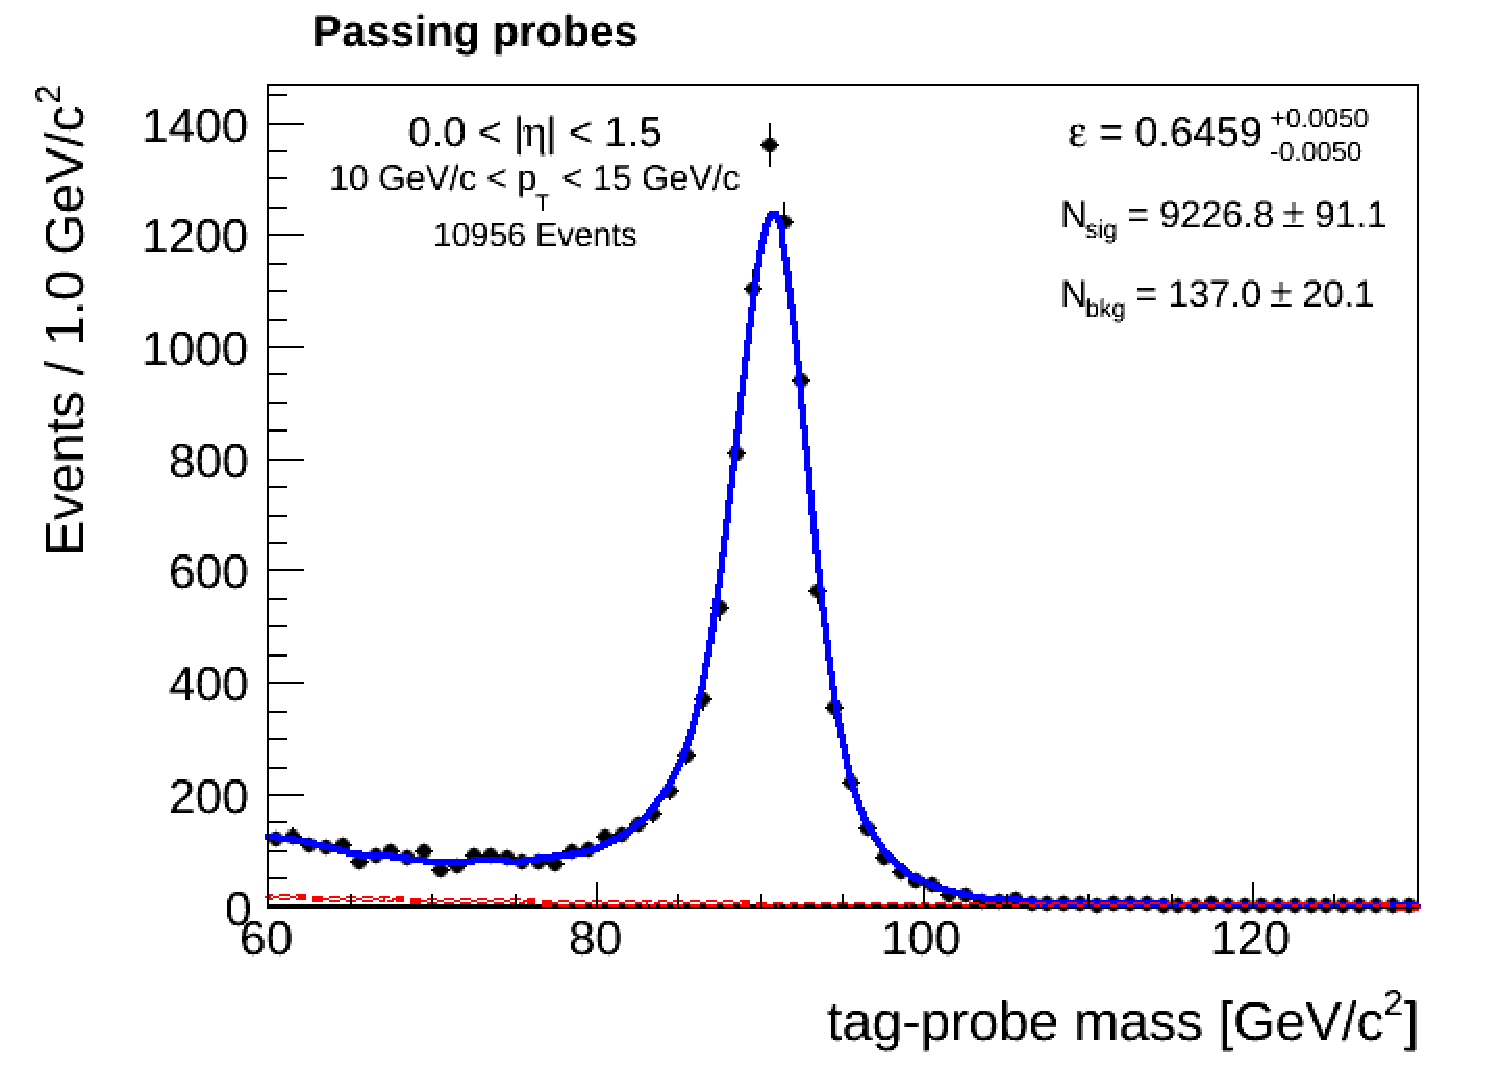
\includegraphics[width=0.45\textwidth]{figures/MuonSelectionEffMassFitPass_EtaPtBin0.pdf}
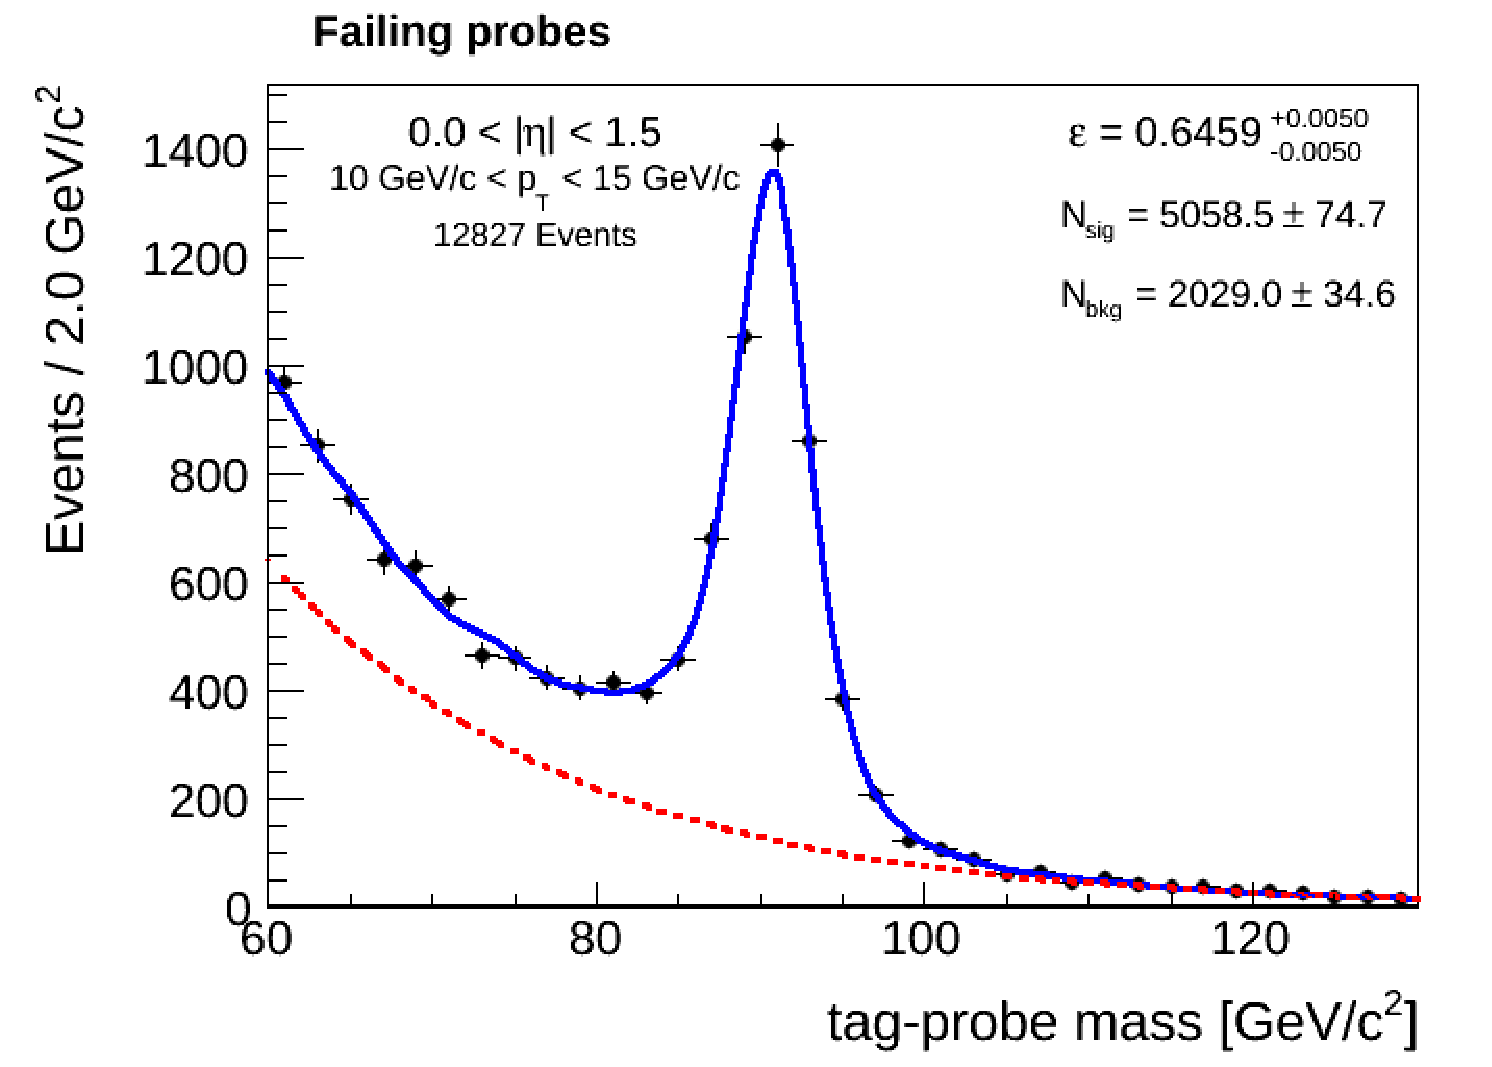
\includegraphics[width=0.45\textwidth]{figures/MuonSelectionEffMassFitFail_EtaPtBin0.pdf}
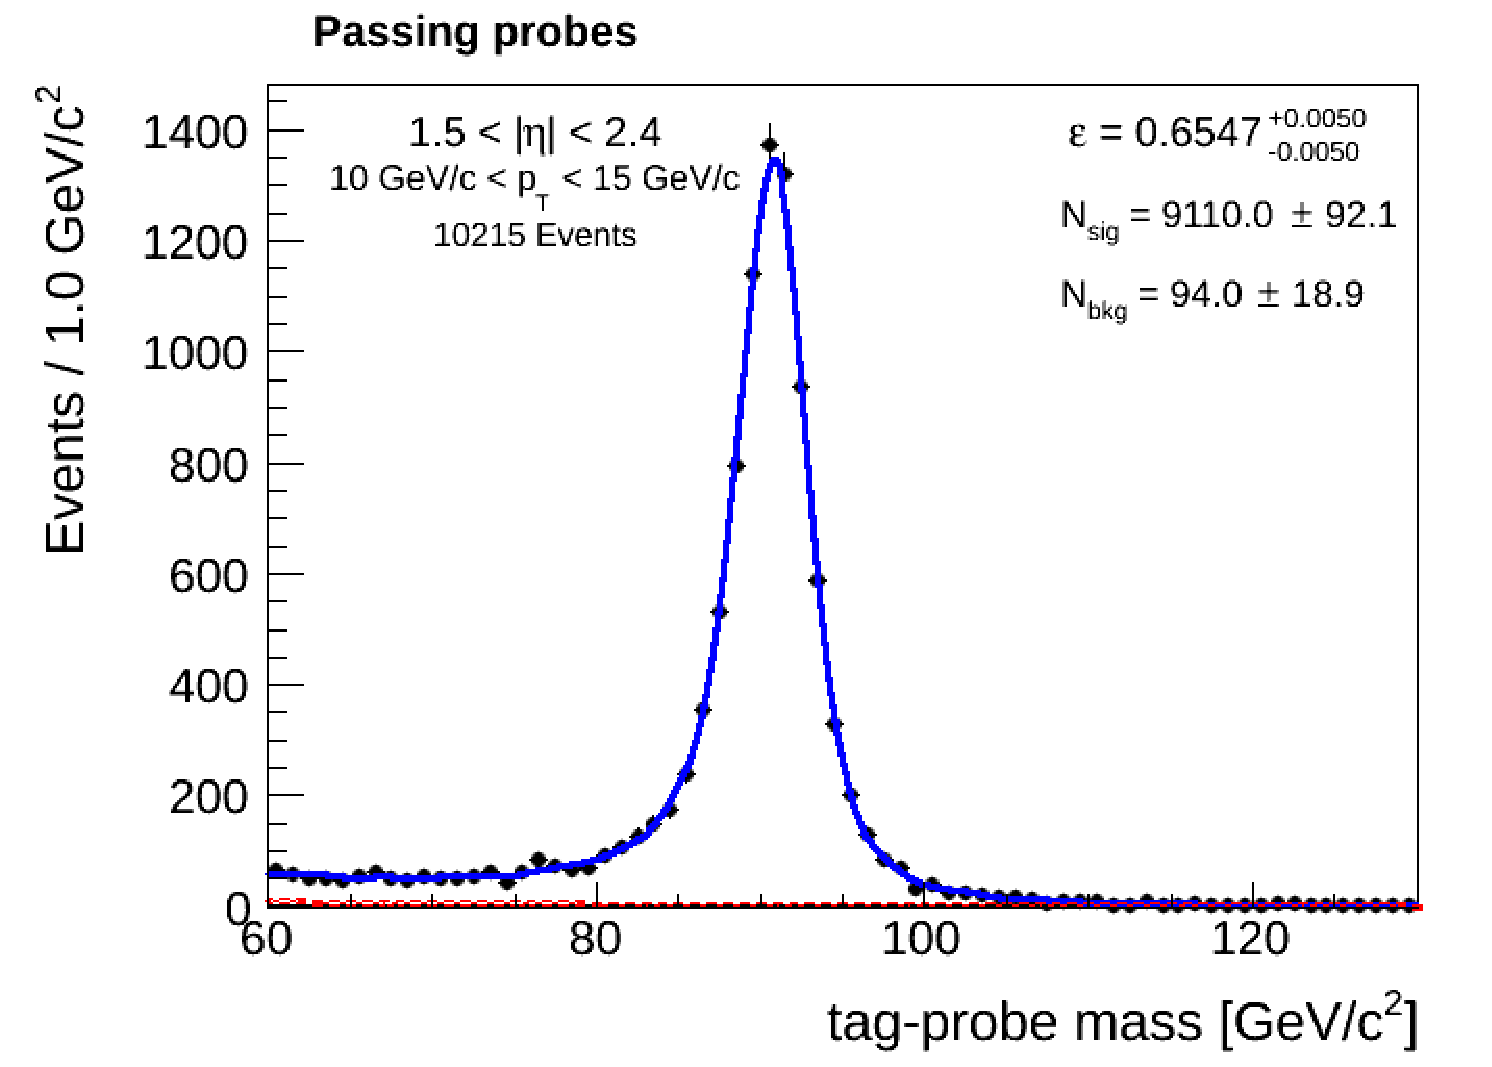
\includegraphics[width=0.45\textwidth]{figures/MuonSelectionEffMassFitPass_EtaPtBin1.pdf}
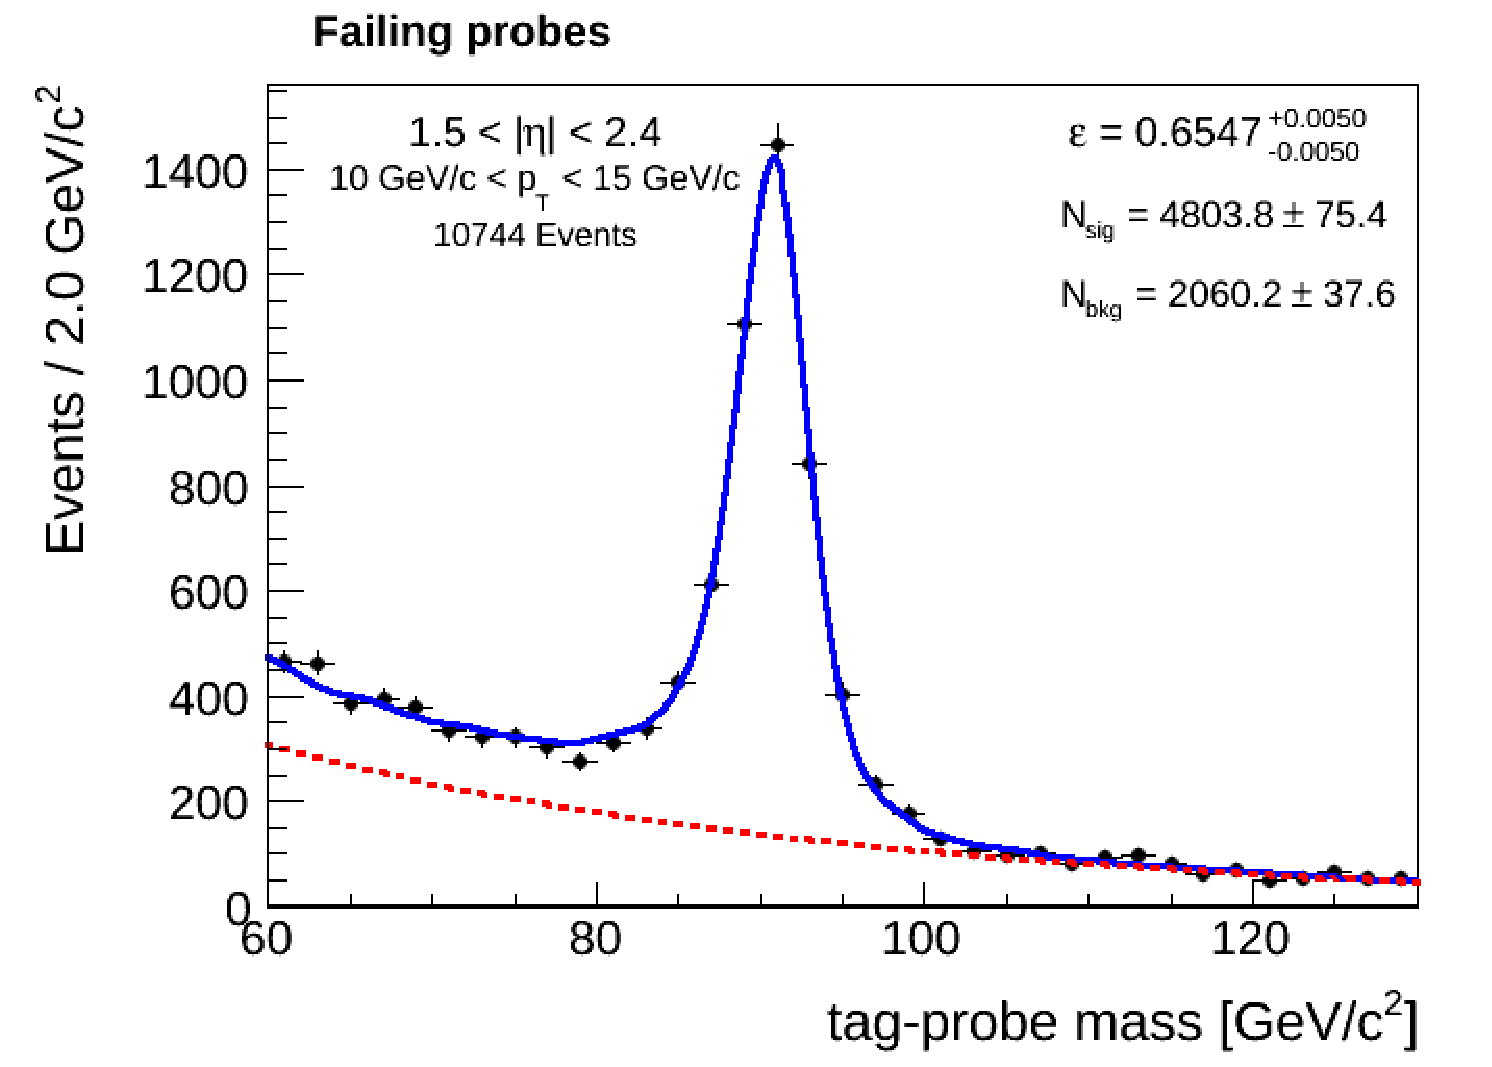
\includegraphics[width=0.45\textwidth]{figures/MuonSelectionEffMassFitFail_EtaPtBin1.pdf}
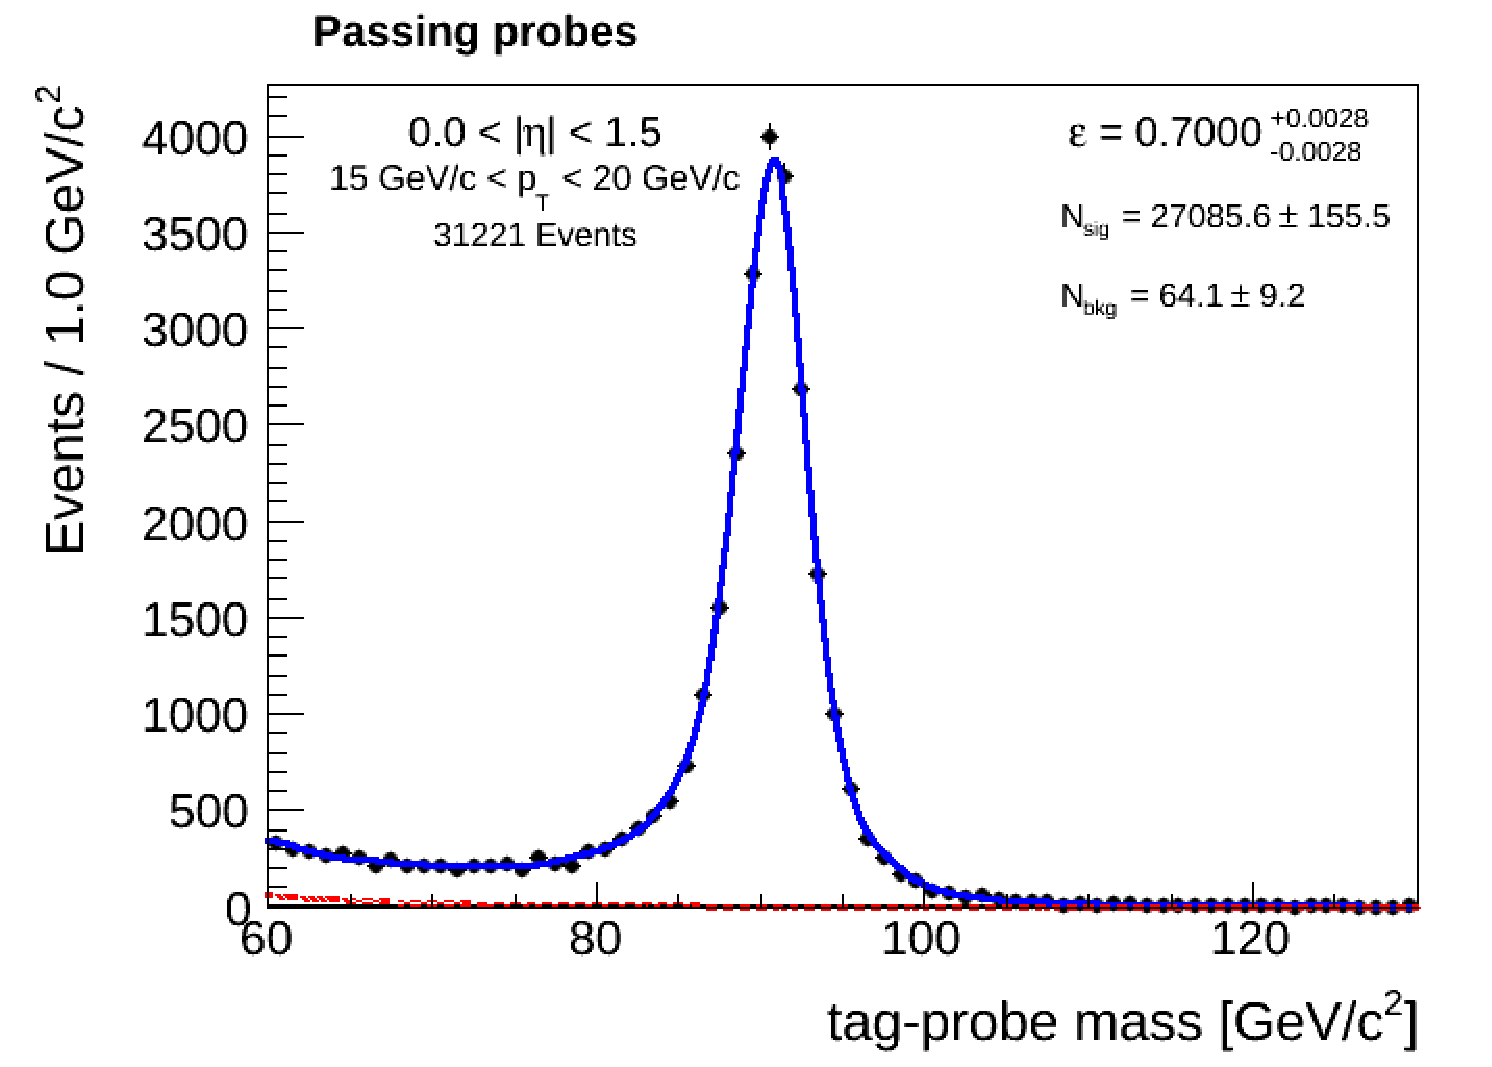
\includegraphics[width=0.45\textwidth]{figures/MuonSelectionEffMassFitPass_EtaPtBin2.pdf}
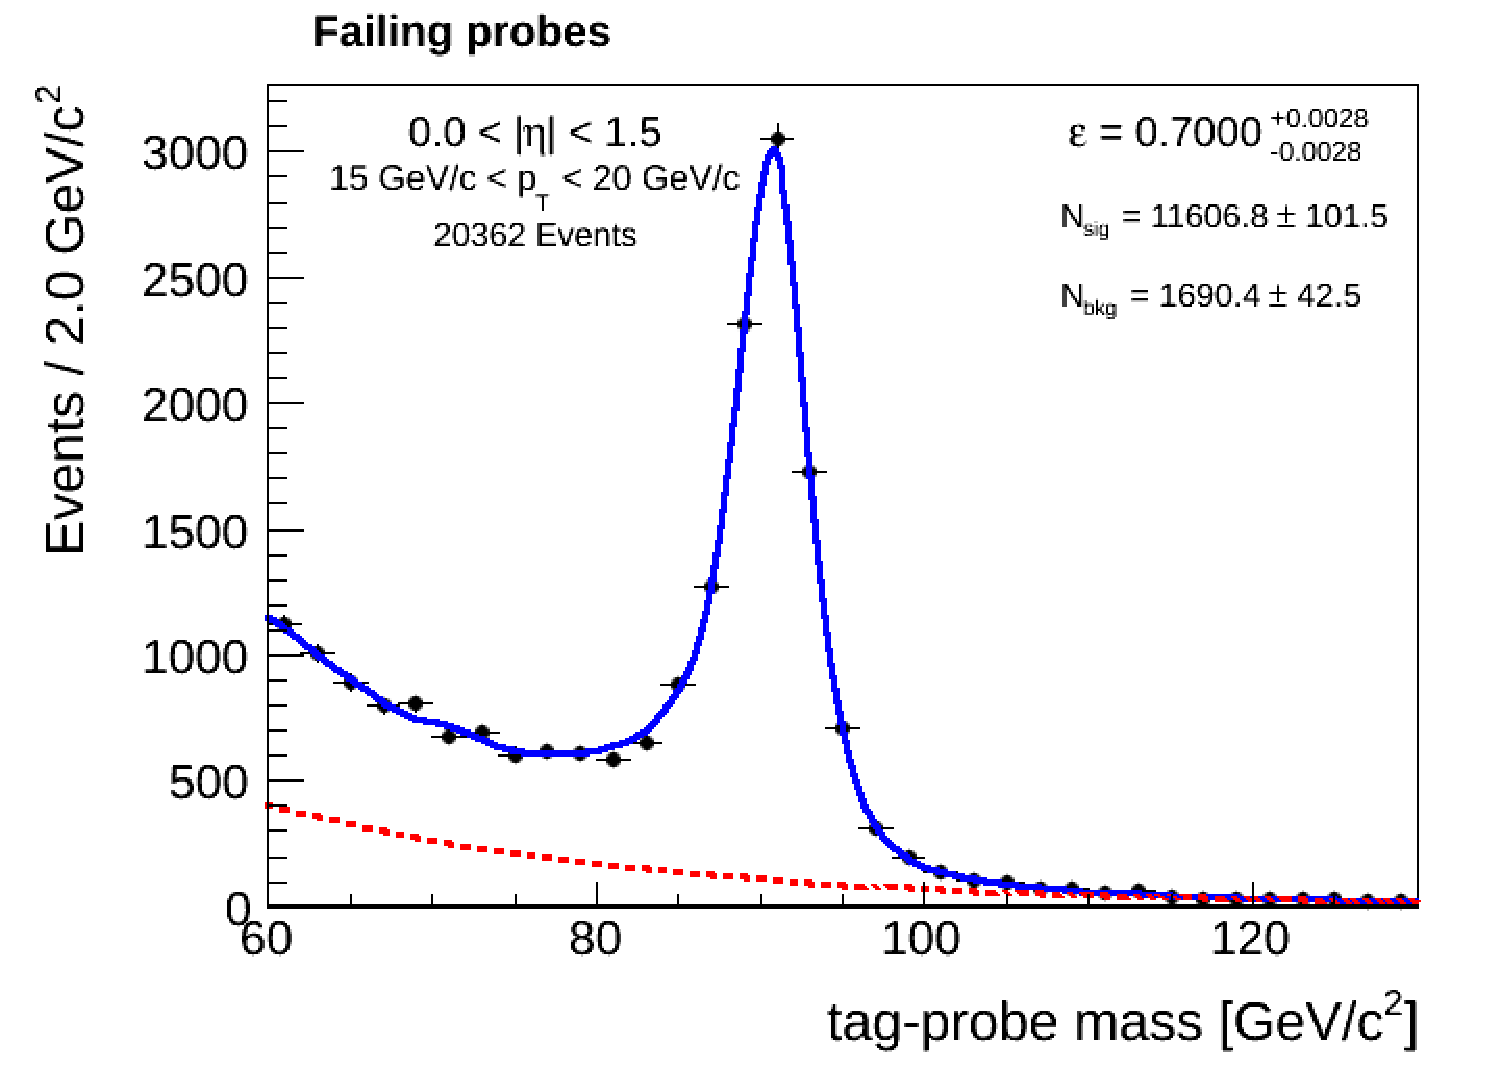
\includegraphics[width=0.45\textwidth]{figures/MuonSelectionEffMassFitFail_EtaPtBin2.pdf}
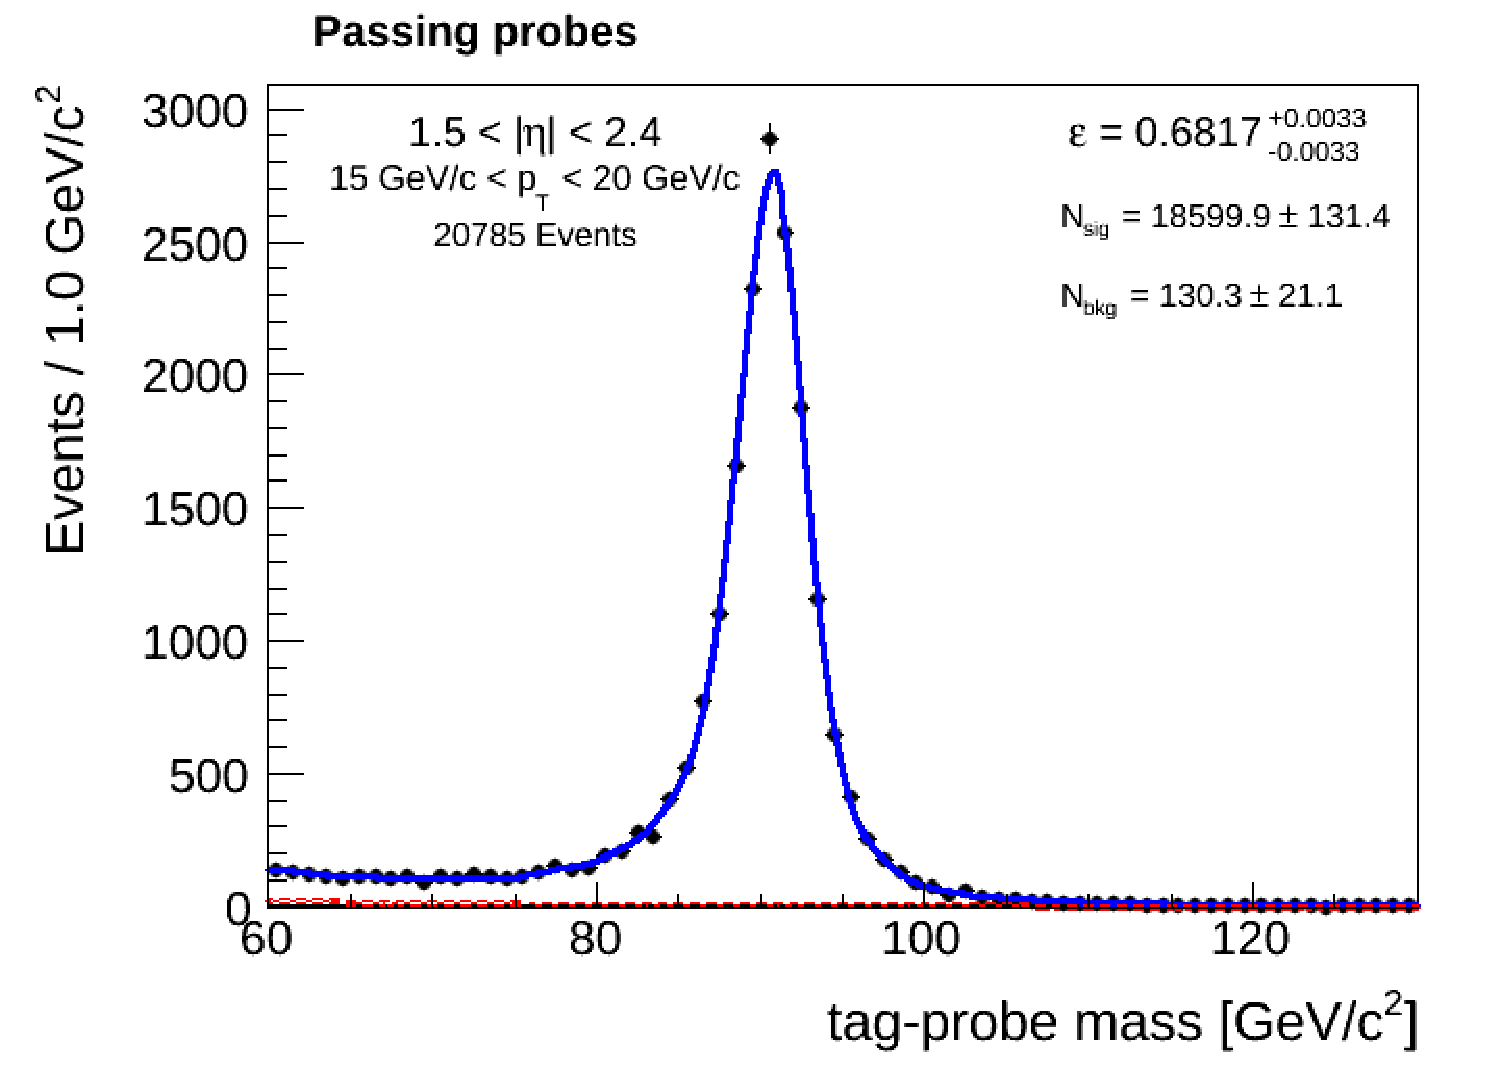
\includegraphics[width=0.45\textwidth]{figures/MuonSelectionEffMassFitPass_EtaPtBin3.pdf}
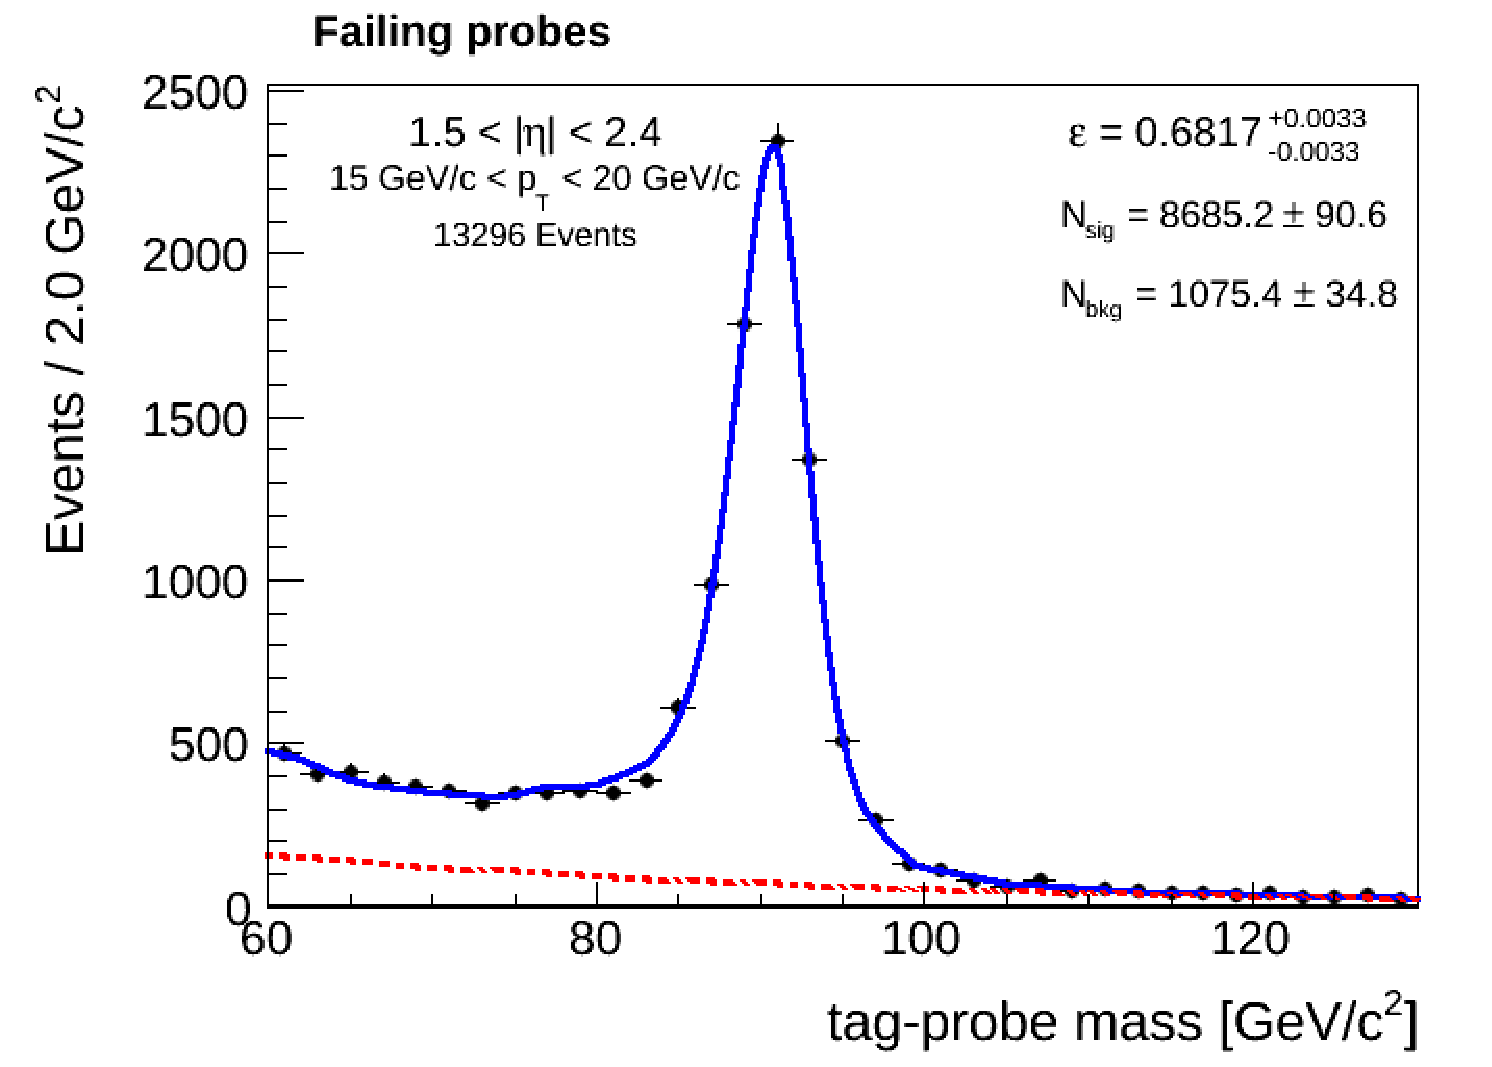
\includegraphics[width=0.45\textwidth]{figures/MuonSelectionEffMassFitFail_EtaPtBin3.pdf}
\caption{Dimuon mass fits for the selection efficiency measurement for muons with
$p_{T}$ less than $20$\GeV.}
\label{fig:mu_selectionEfficiency_massfits_lowPt}
\end{center}
\end{figure}

\begin{figure}[!htbp]
\begin{center}
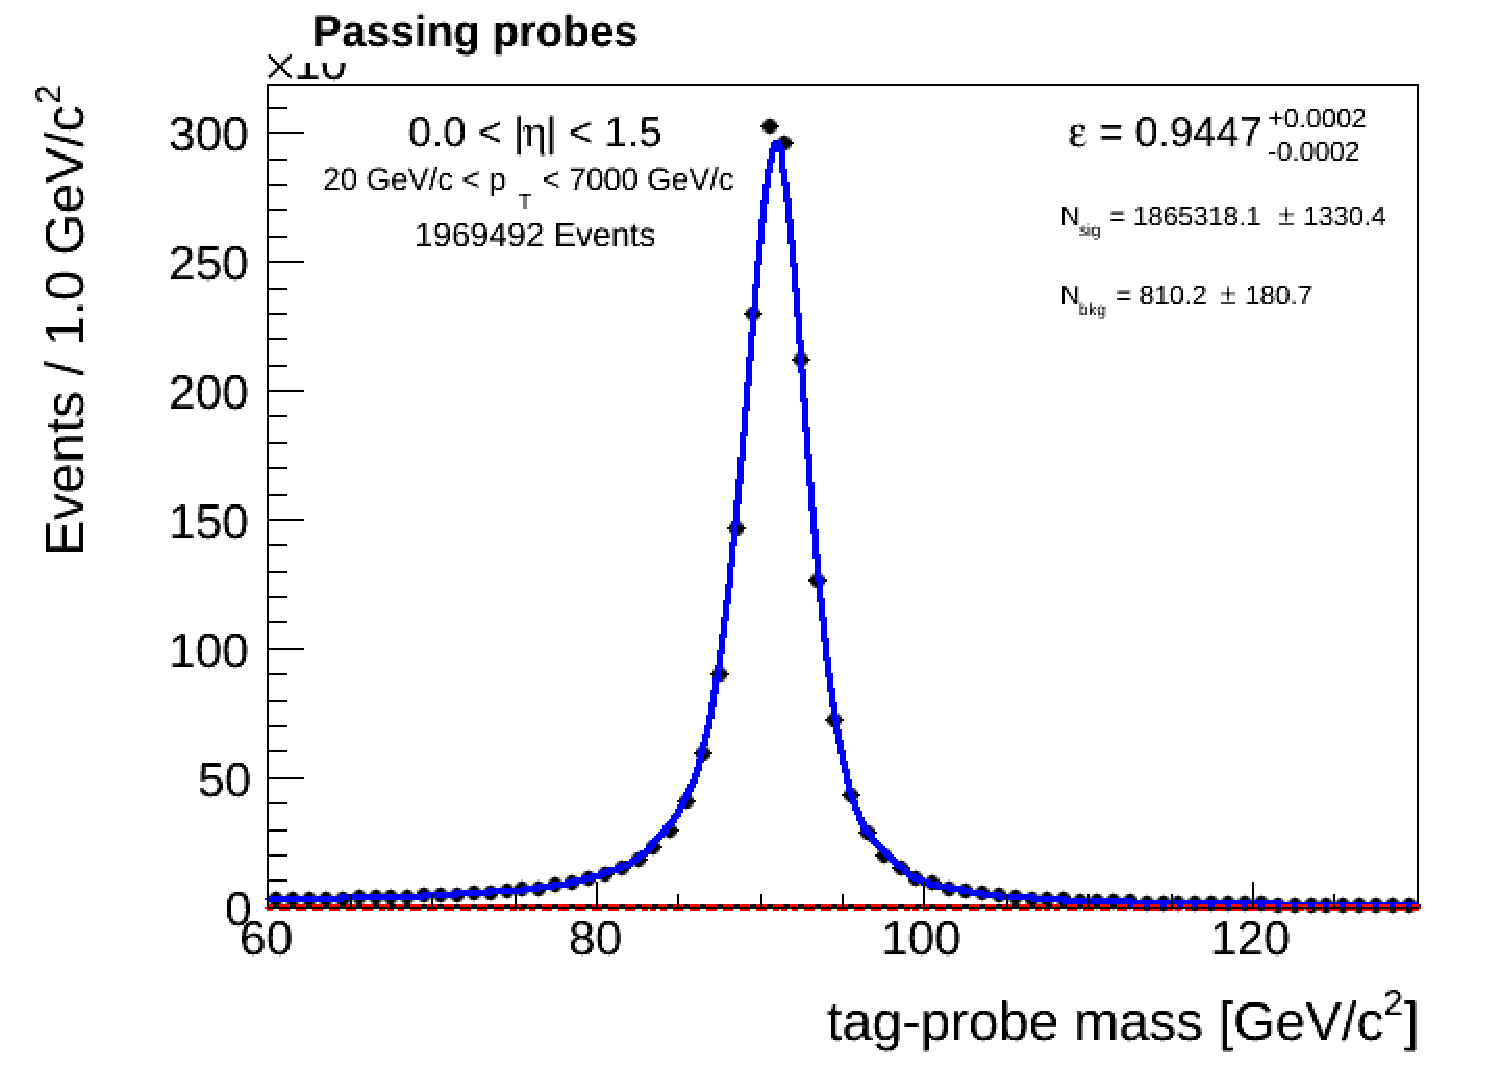
\includegraphics[width=0.45\textwidth]{figures/MuonSelectionEffMassFitPass_EtaPtBin4.pdf}
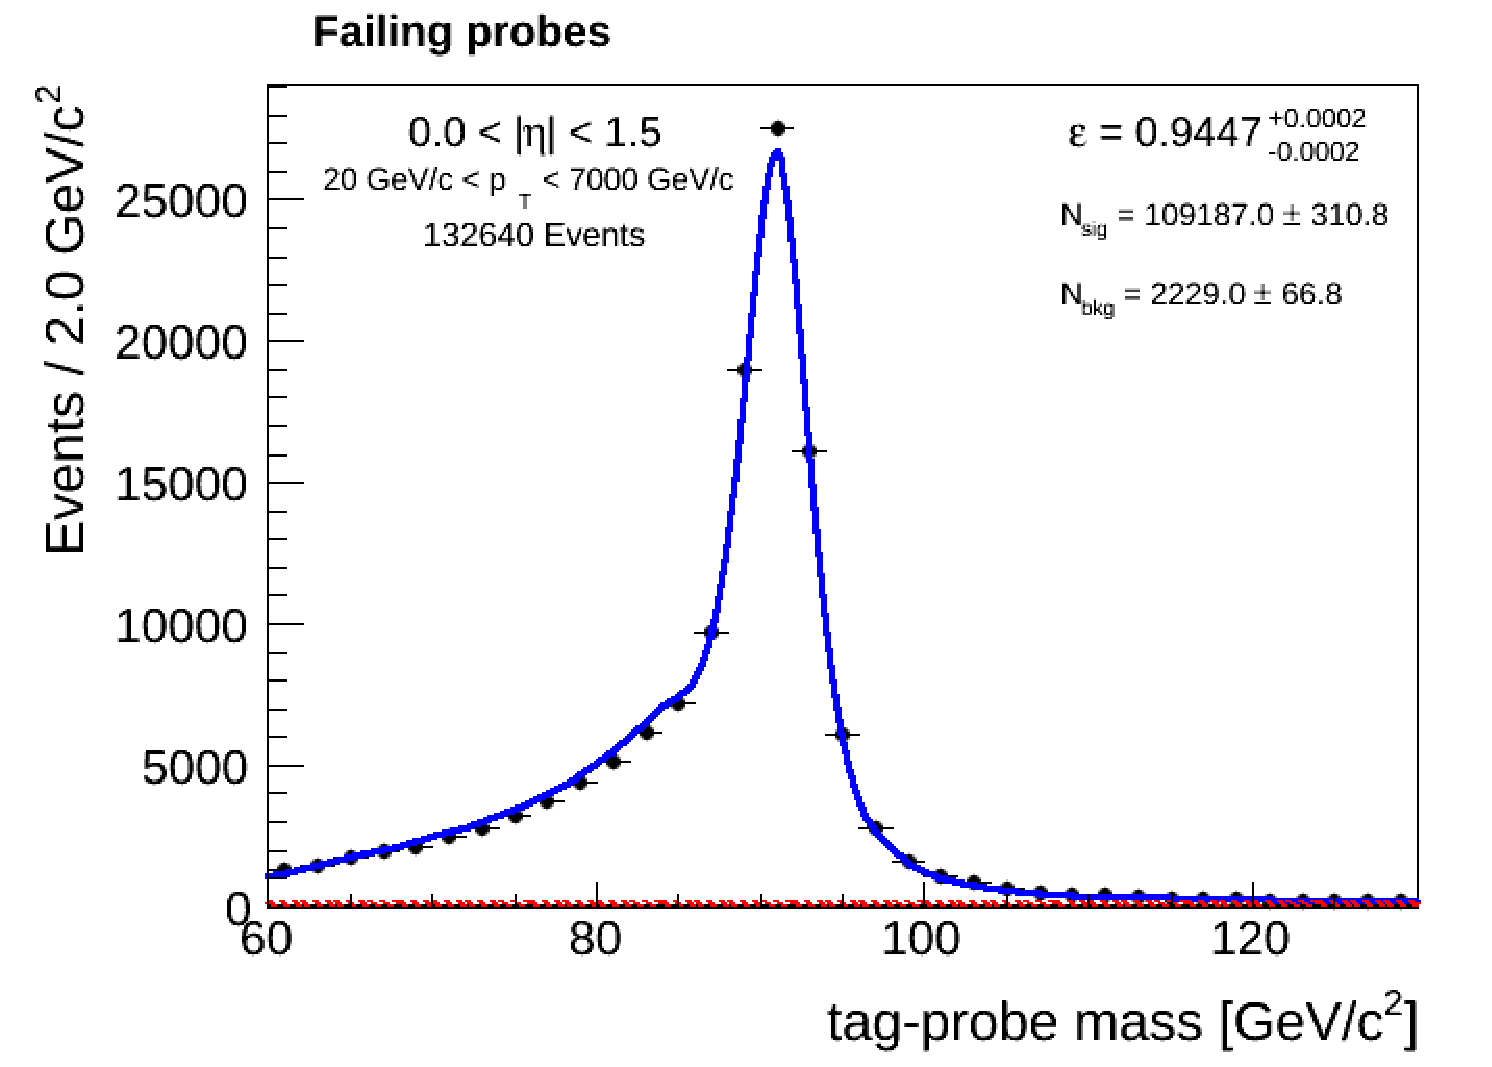
\includegraphics[width=0.45\textwidth]{figures/MuonSelectionEffMassFitFail_EtaPtBin4.pdf}
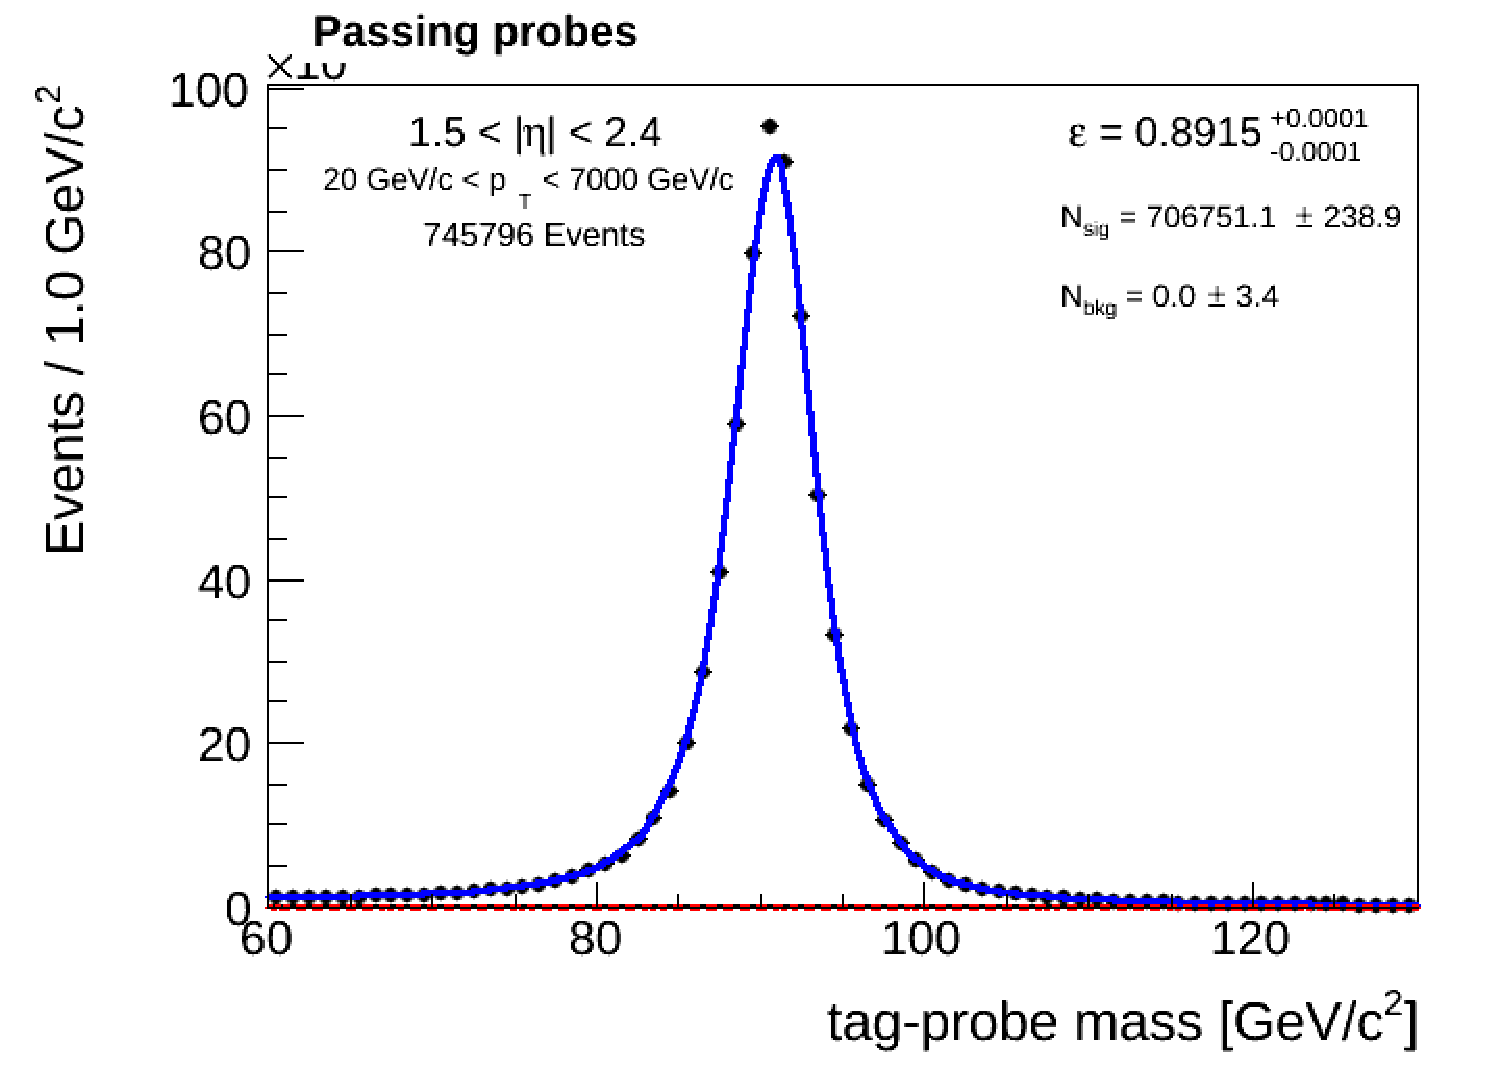
\includegraphics[width=0.45\textwidth]{figures/MuonSelectionEffMassFitPass_EtaPtBin5.pdf}
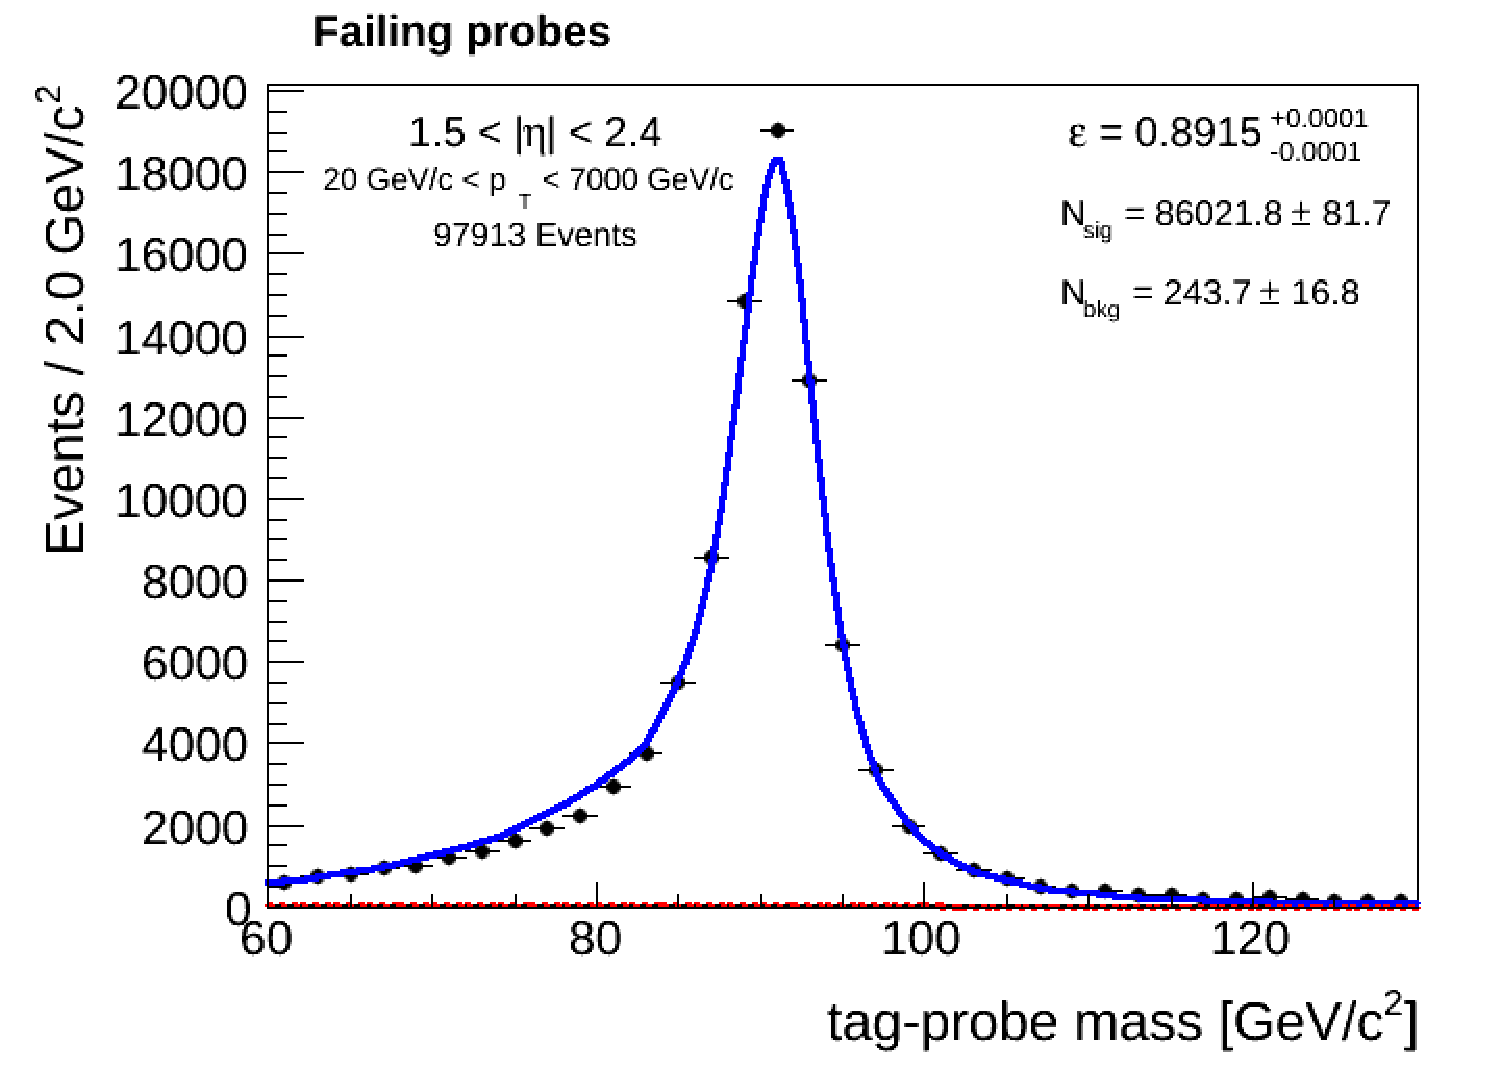
\includegraphics[width=0.45\textwidth]{figures/MuonSelectionEffMassFitFail_EtaPtBin5.pdf}
\caption{Dimuon mass fits for the selection efficiency measurement for muons with
$p_{T}$ greater than $20$\GeV.}
\label{fig:mu_selectionEfficiency_massfits_highPt}
\end{center}
\end{figure}


The muon selection efficiency is plotted as a function of the $p_{T}$ of the muon in Figure 
\ref{fig:mu_selectionEfficiency_VsPt} and as a function of the pseudorapidity of the muon
in Figure \ref{fig:mu_selectionEfficiency_VsEta} for low $p_{T}$ and high $p_{T}$ muons separately. Finally in Figures
\ref{fig:mu_selectionEfficiency_LowPt_VsPileup} and \ref{fig:mu_selectionEfficiency_HighPt_VsPileup}
we show the dependence of the efficiency on the amount of pileup, characterized by the
number of primary vertices reconstructed in the event and the pileup energy density 
in the event for low $p_{T}$ and high $p_{T}$ muons respectively.

\begin{figure}[!htbp]
\begin{center}
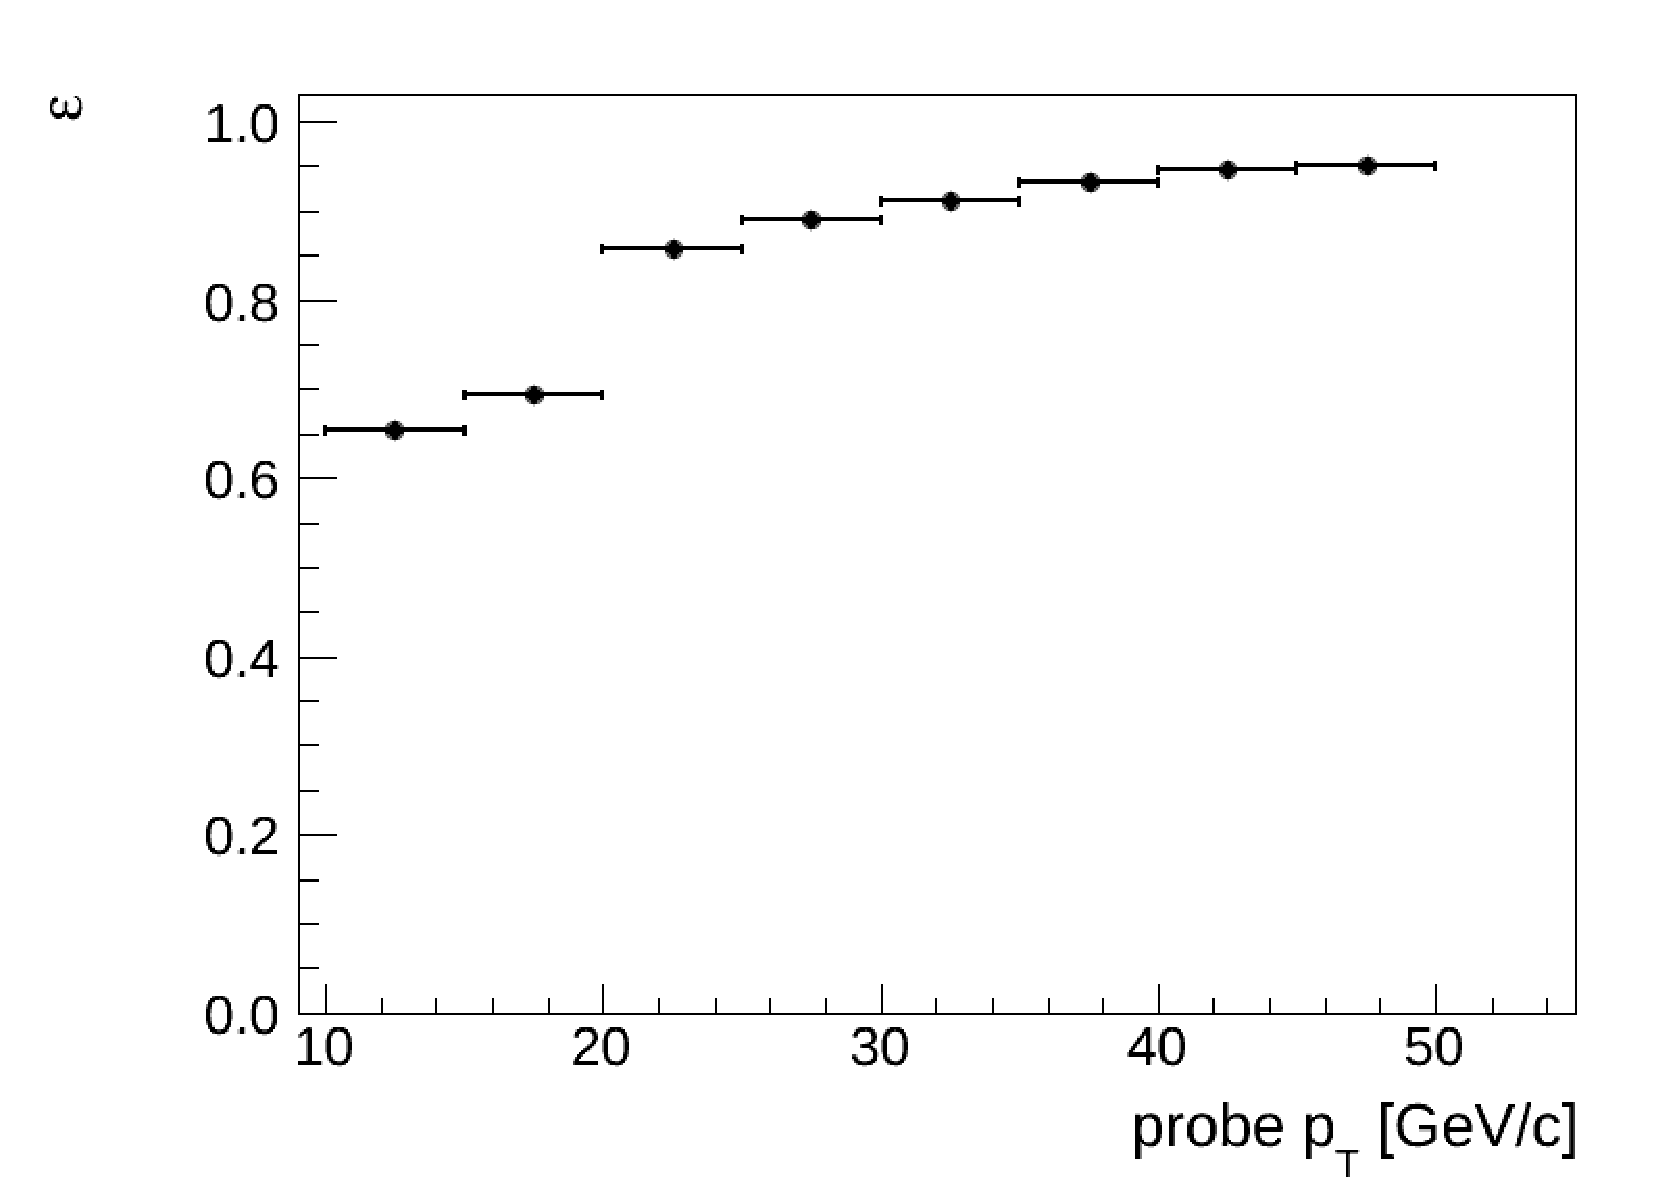
\includegraphics[width=0.45\textwidth]{figures/MuonEff_VsPt.pdf}
\caption{Muon selection efficiency as a function of the $p_{T}$ of the muon.}
\label{fig:mu_selectionEfficiency_VsPt}
\end{center}
\end{figure}


\begin{figure}[!htbp]
\begin{center}
\subfigure[$10$ \GeV\ $ < p_{T} \le 20$ \GeV]{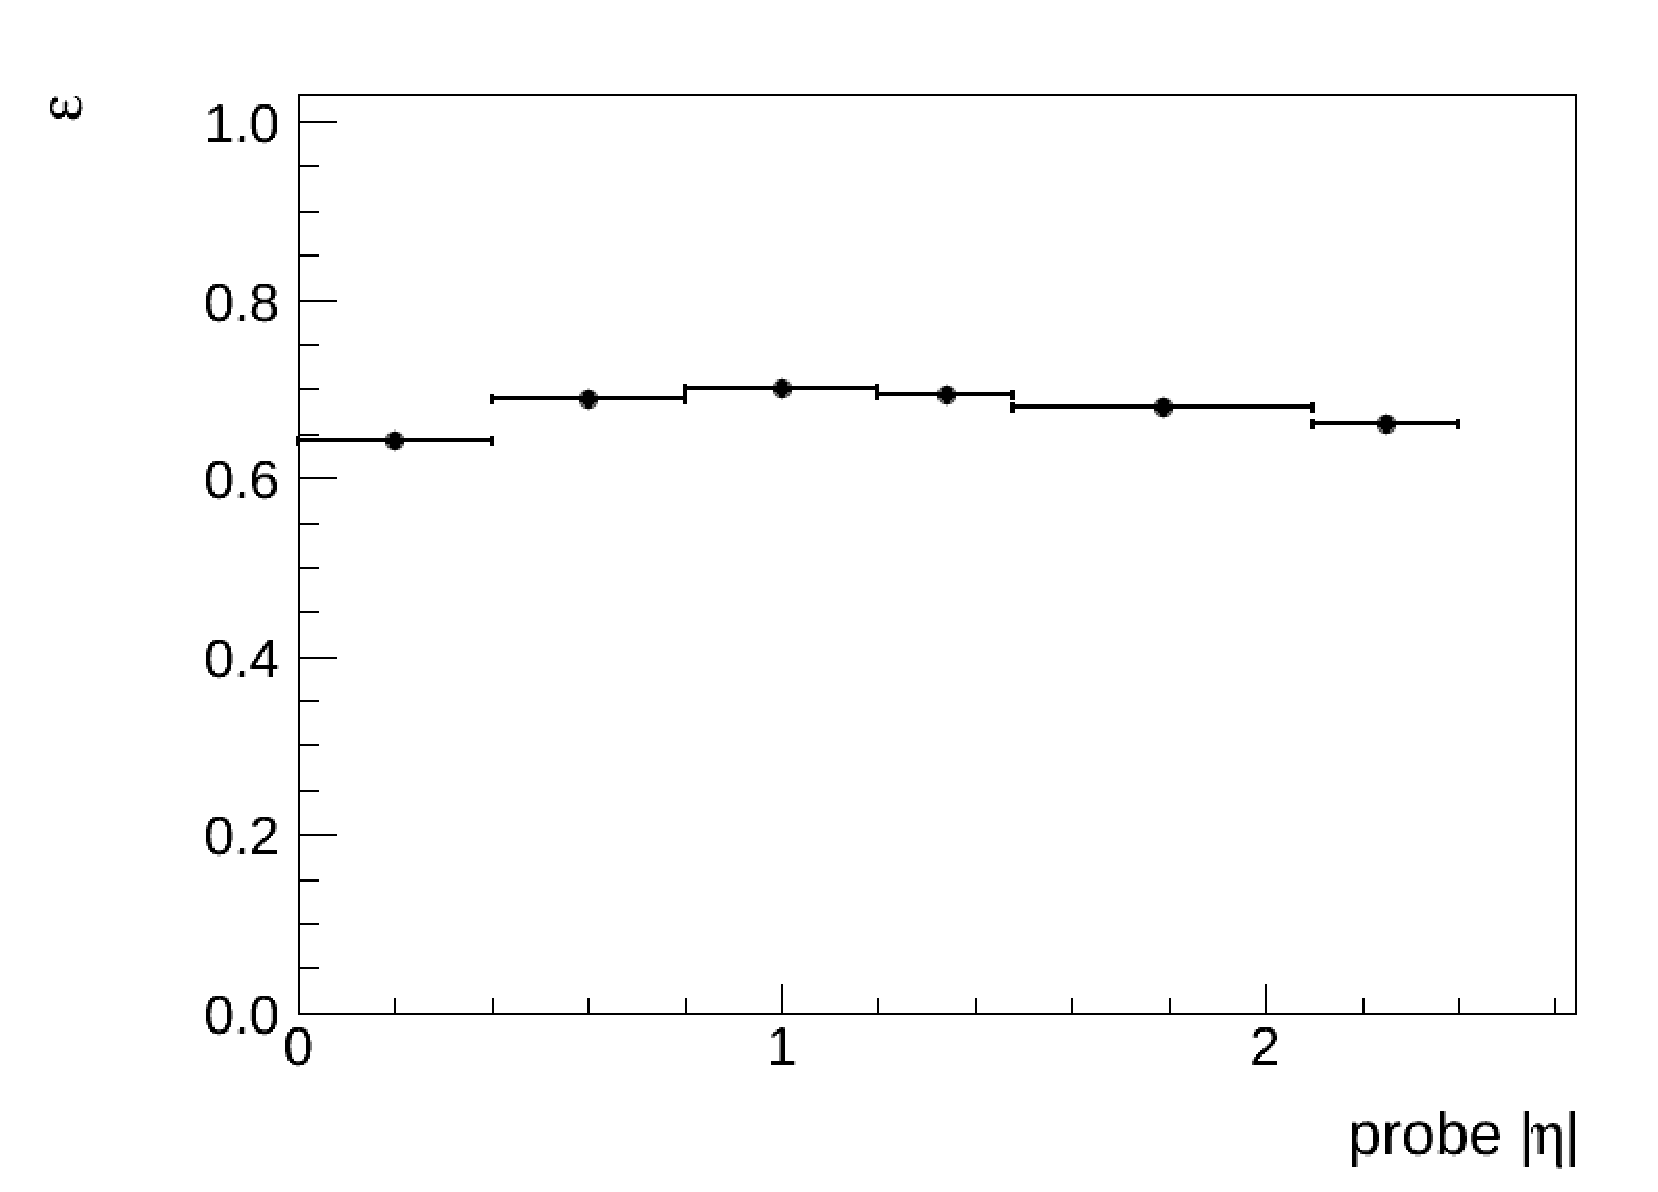
\includegraphics[width=0.45\textwidth]{figures/MuonEff_LowPt_VsEta.pdf}}
\subfigure[$p_{T} > 20$]{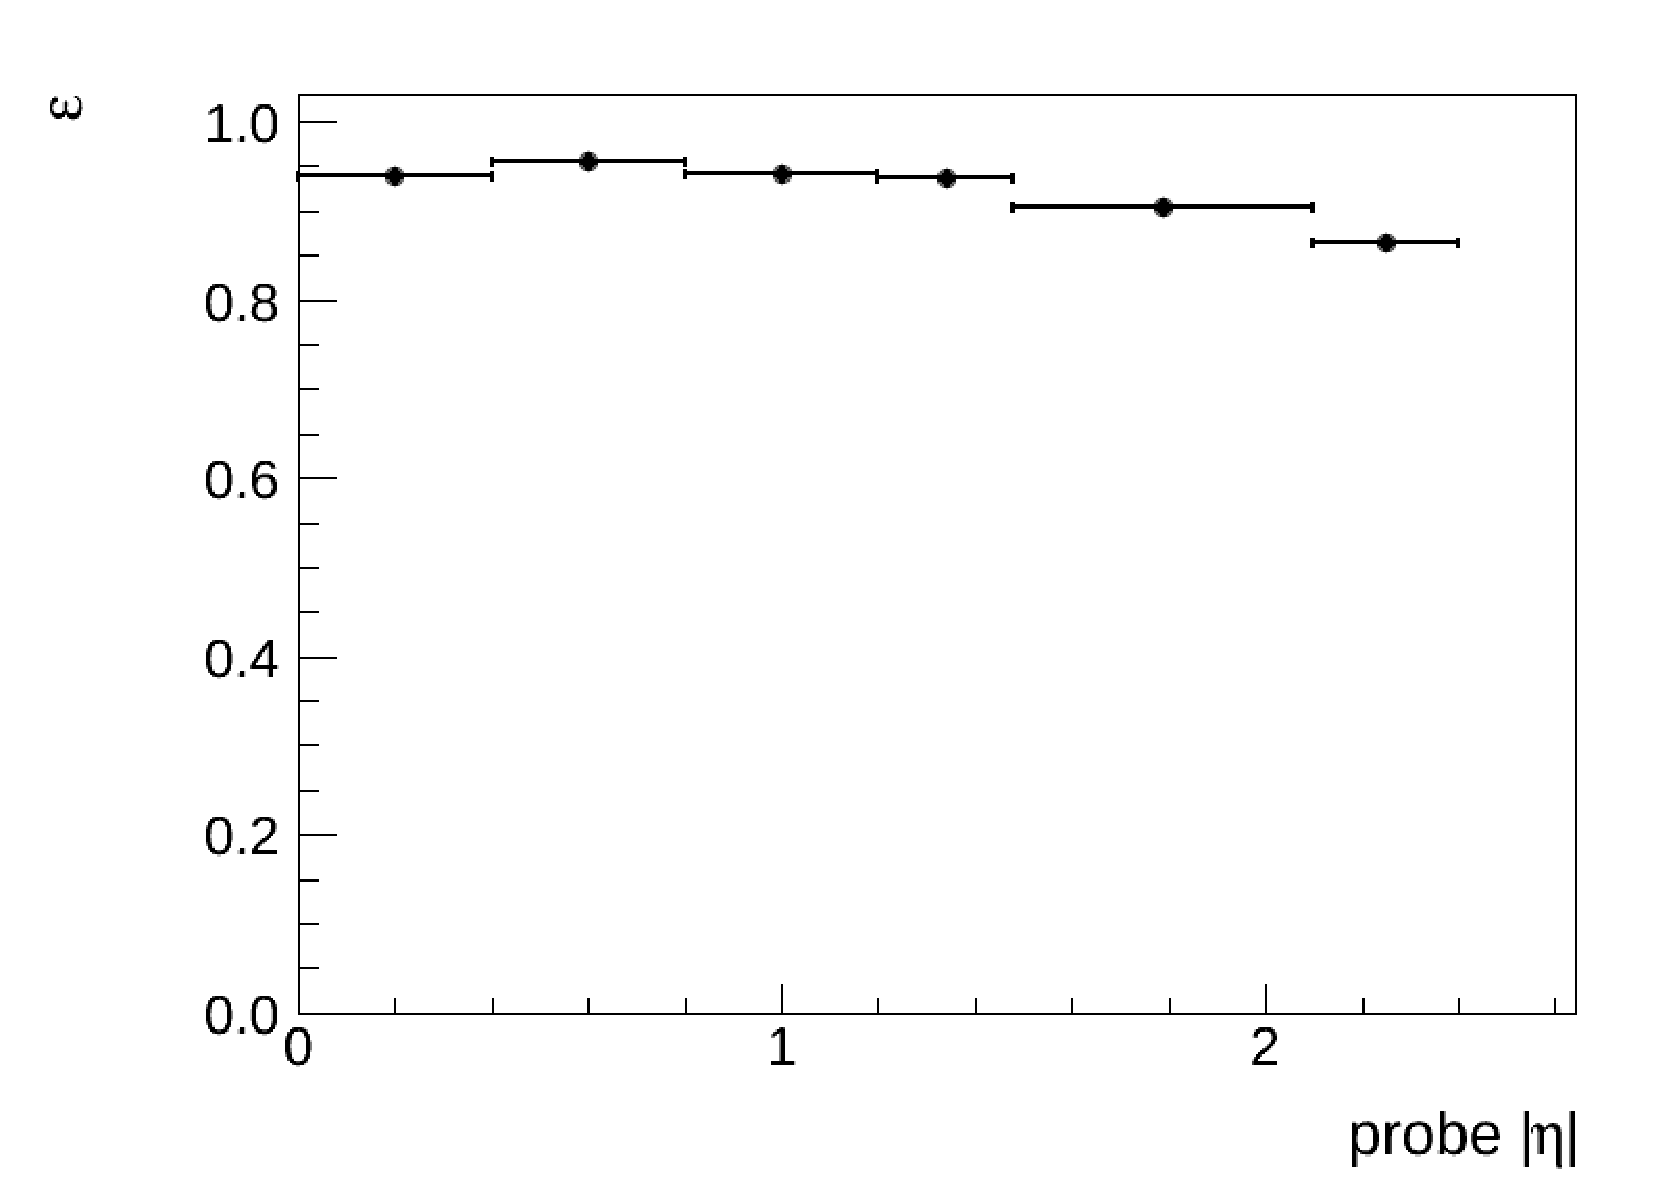
\includegraphics[width=0.45\textwidth]{figures/MuonEff_HighPt_VsEta.pdf}}
\caption{Muon selection efficiency as a function of the $p_{T}$ of the muon.}
\label{fig:mu_selectionEfficiency_VsEta}
\end{center}
\end{figure}



\begin{figure}[!htbp]
\begin{center}
\subfigure[Number of reconstructed primary vertices]{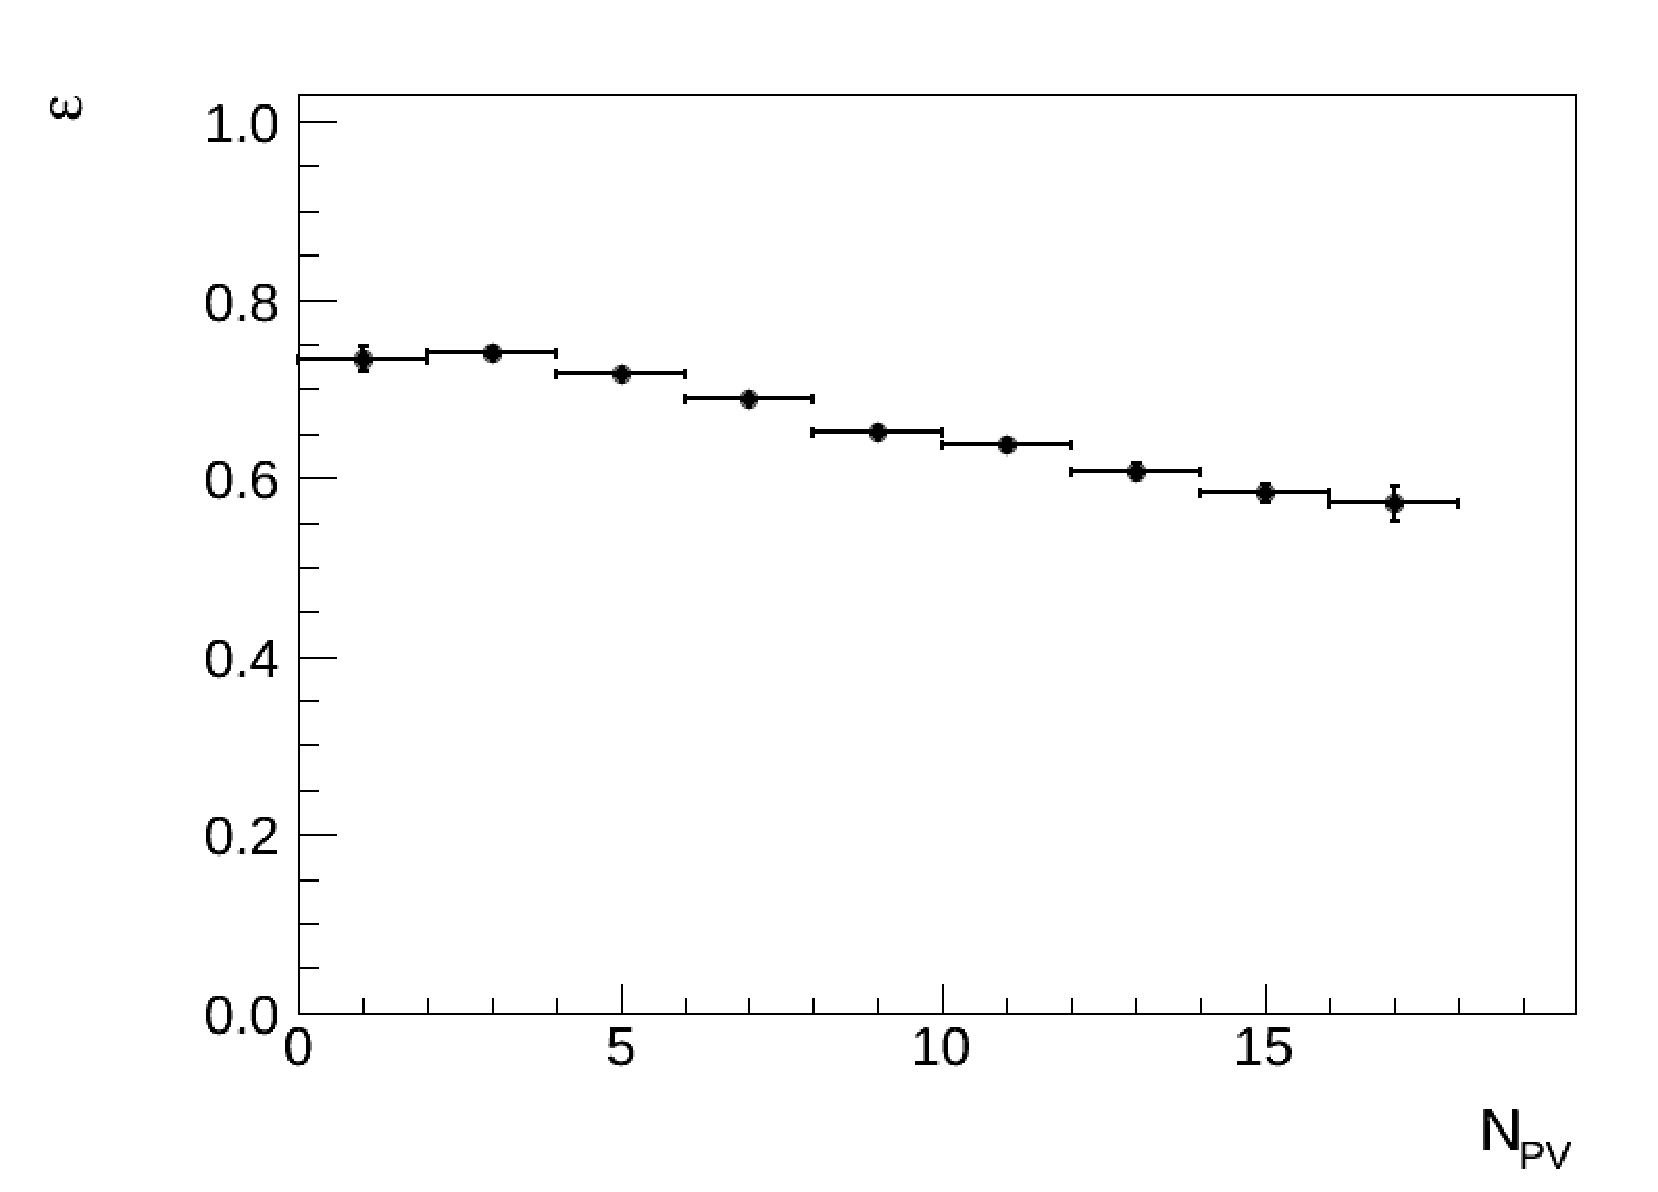
\includegraphics[width=0.45\textwidth]{figures/MuonEff_LowPt_VsNVtx.pdf}}
\subfigure[Pileup energy density ($\rho$)]{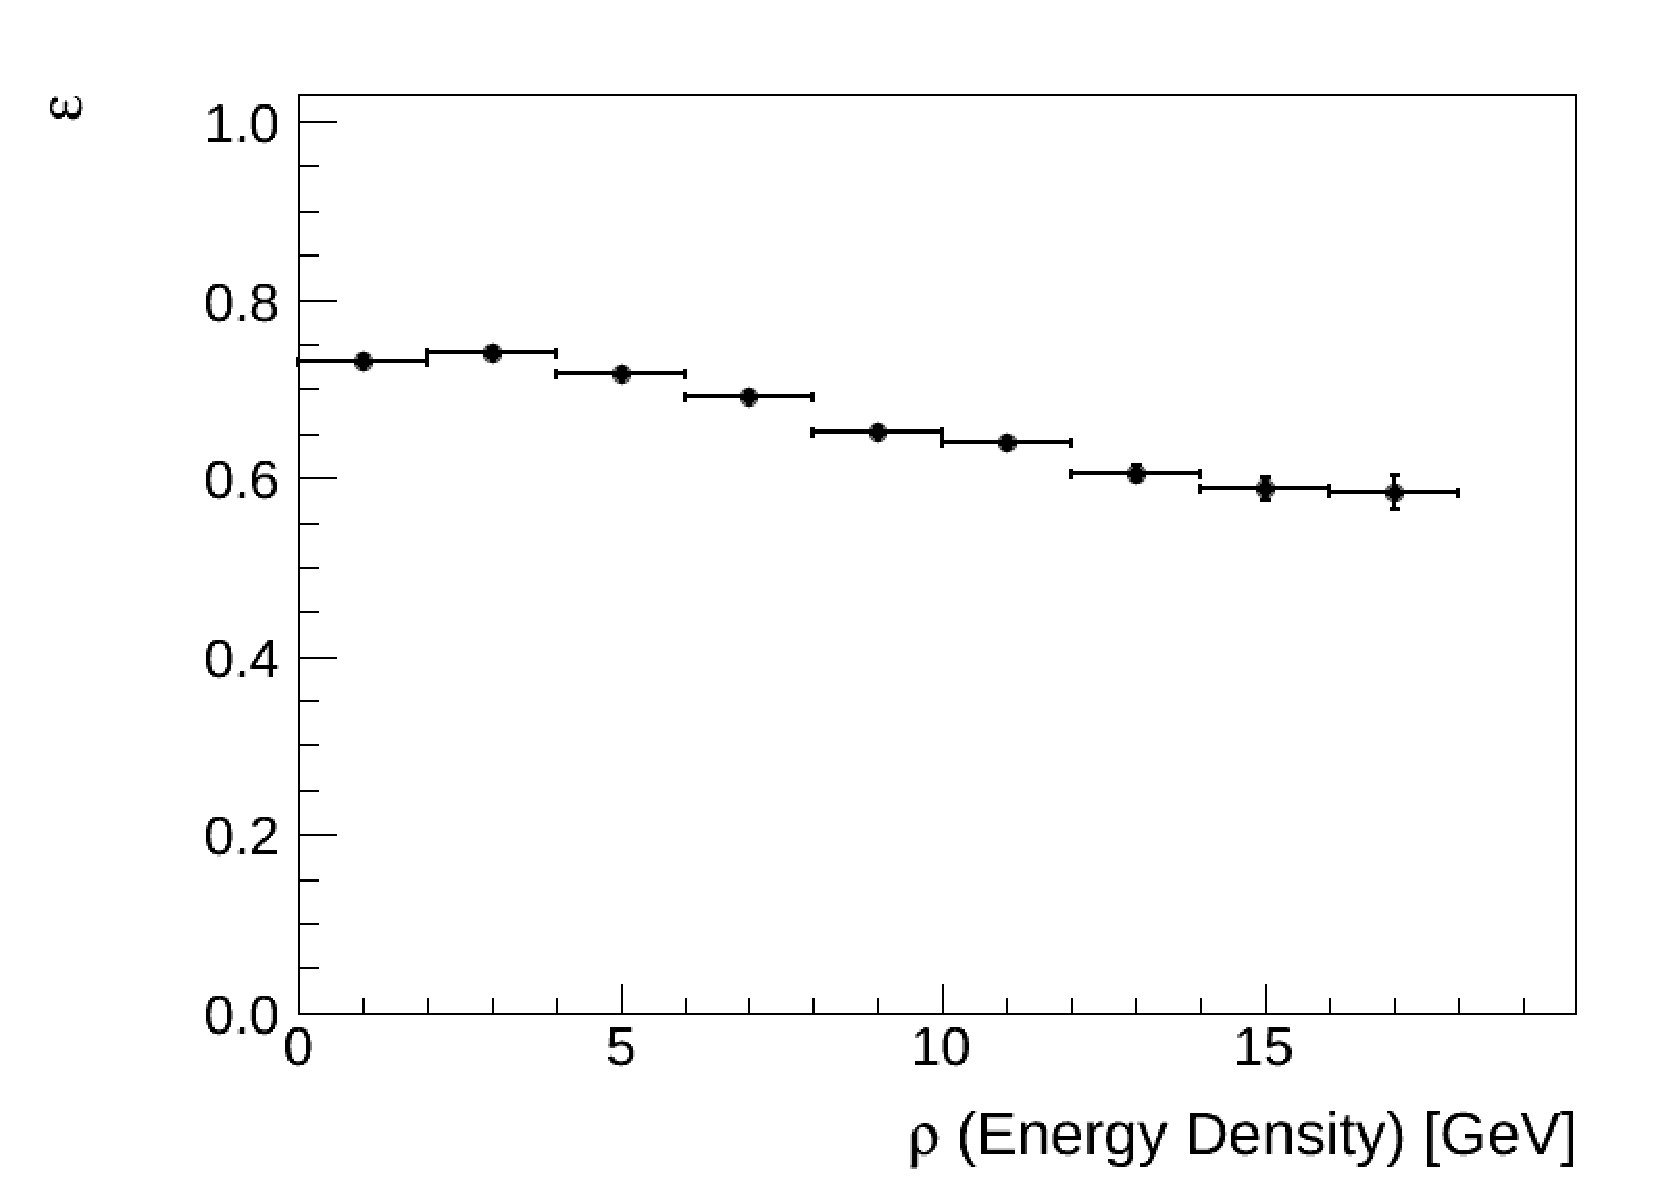
\includegraphics[width=0.45\textwidth]{figures/MuonEff_LowPt_VsRho.pdf}}
\caption{Muon selection efficiency as a function of the number of reconstructed primary vertices
and the pileup energy density for muons with $p_{T}$ between 10 and 20\GeV.}
\label{fig:mu_selectionEfficiency_LowPt_VsPileup}
\end{center}
\end{figure}



\begin{figure}[!htbp]
\begin{center}
\subfigure[Number of reconstructed primary vertices]{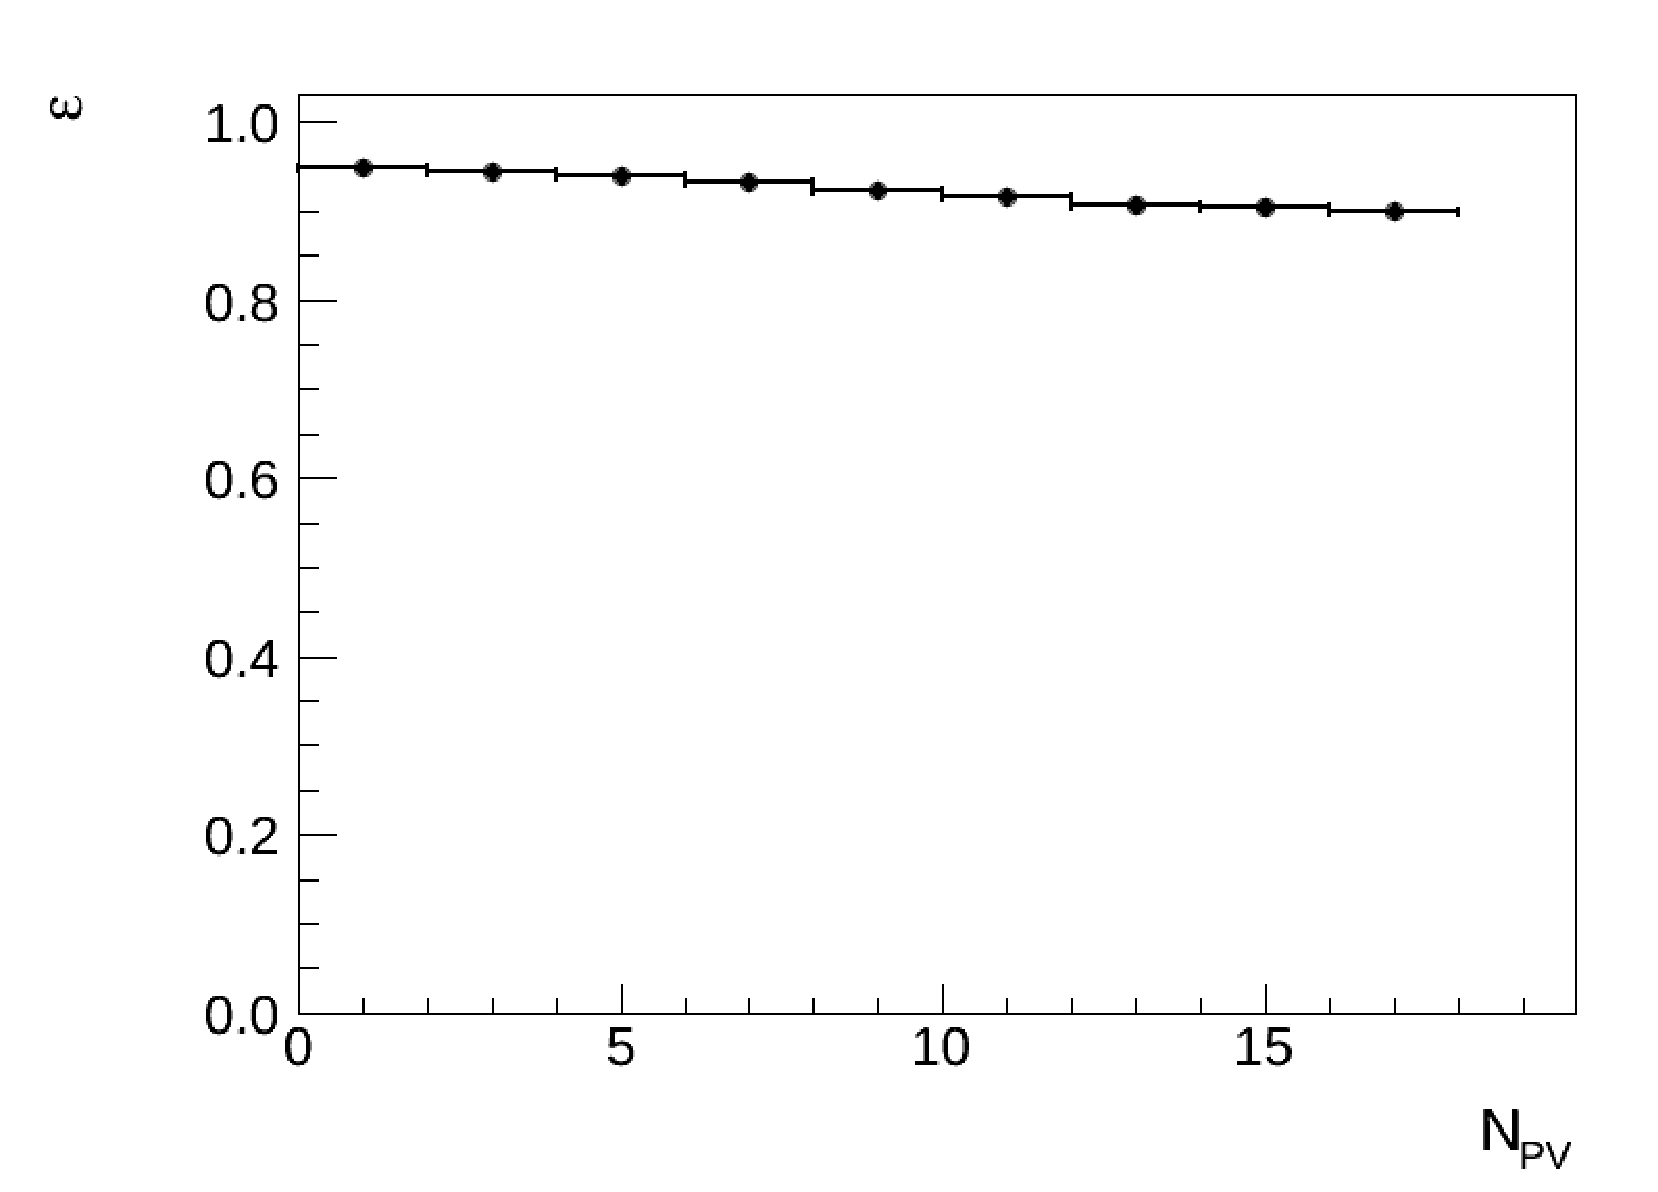
\includegraphics[width=0.45\textwidth]{figures/MuonEff_HighPt_VsNVtx.pdf}}
\subfigure[Pileup energy density ($\rho$)]{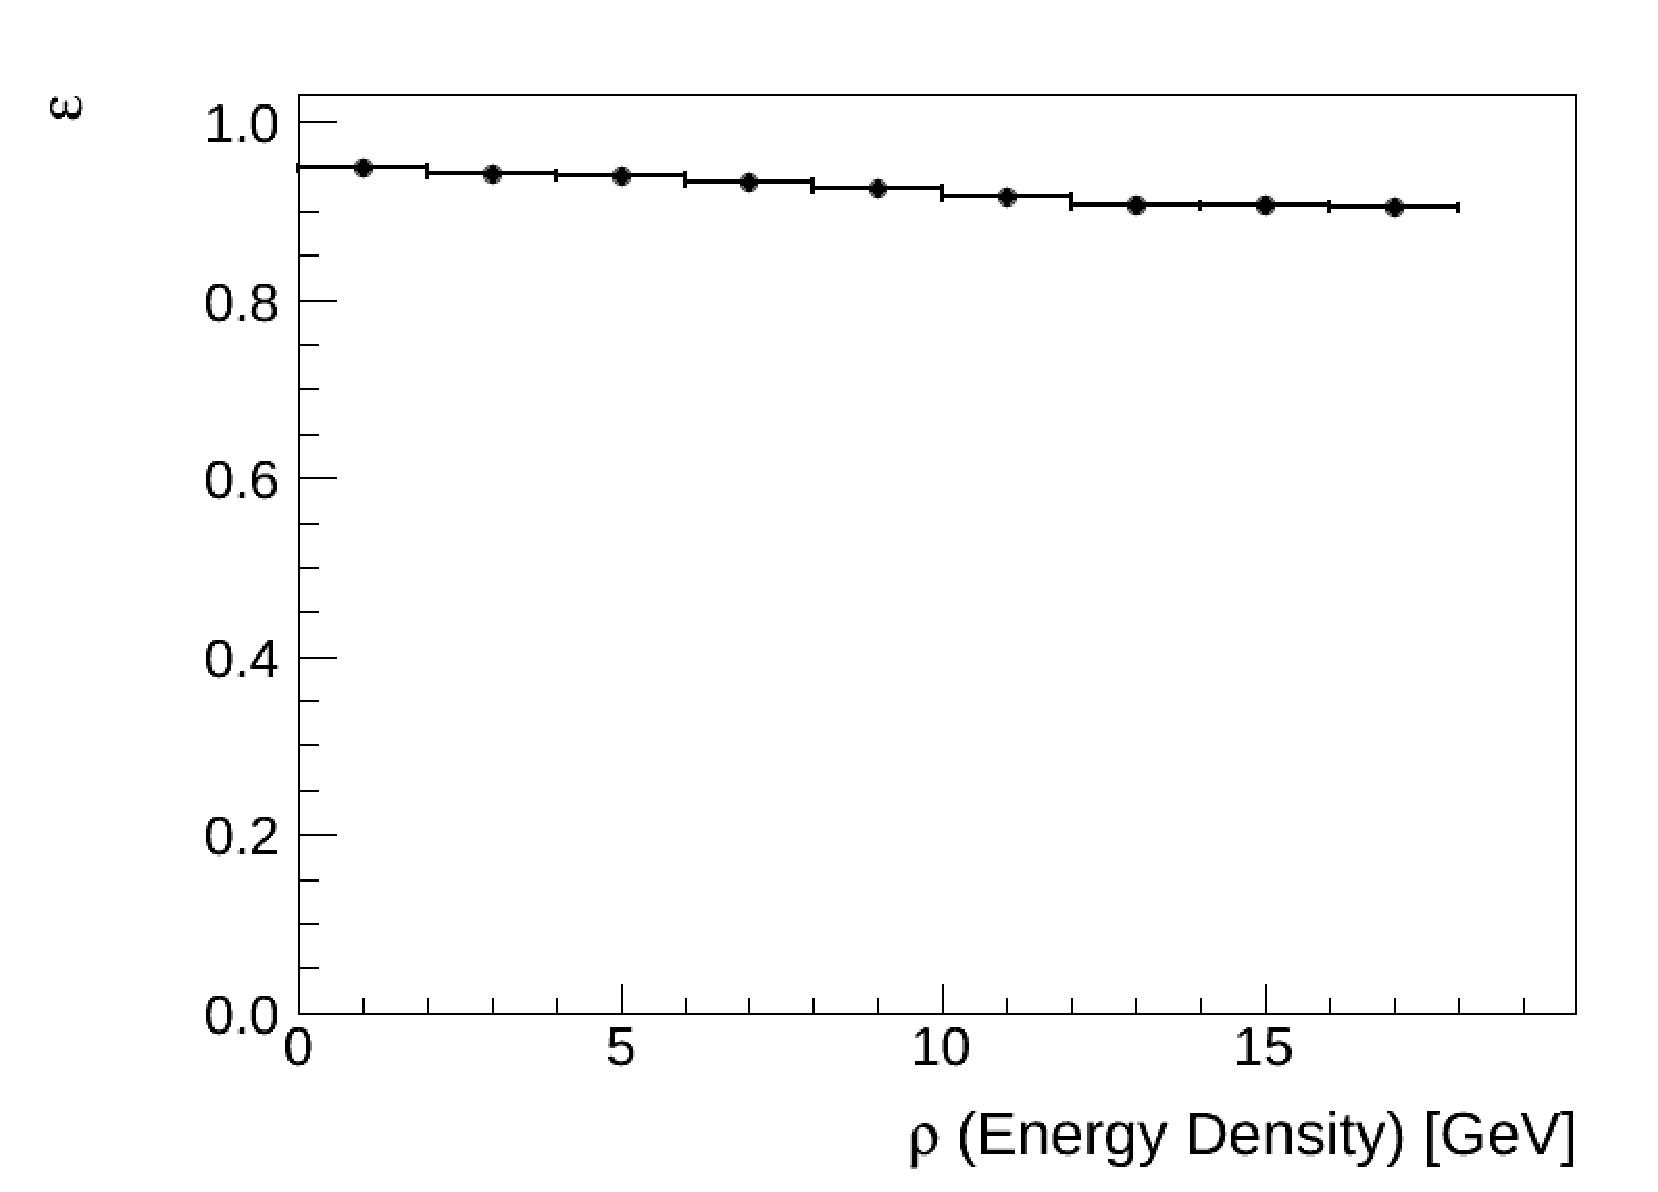
\includegraphics[width=0.45\textwidth]{figures/MuonEff_HighPt_VsRho.pdf}}
\caption{Muon selection efficiency as a function of the number of reconstructed primary vertices
and the pileup energy density for muons with $p_{T}$ greater than 20\GeV.}
\label{fig:mu_selectionEfficiency_HighPt_VsPileup}
\end{center}
\end{figure}



